\documentclass[a4paper,11pt]{article}
\usepackage[hidelinks]{hyperref}
\usepackage{listings} % for code
\usepackage{graphicx}
\usepackage{tikz}
\usetikzlibrary{positioning}
\usetikzlibrary{decorations.pathreplacing}
\usetikzlibrary{calc}
\usepackage{subcaption}
\usepackage{wrapfig}
\usepackage{enumitem}
\usepackage{algorithm}
\usepackage{algorithmicx}
\usepackage{algpseudocode}

\usepackage{amssymb}
\usepackage[mathscr]{euscript}
\usepackage{mathtools}
\usepackage{amsmath}

%% Start of own commands
\algnewcommand\algorithmicinput{\textbf{Input:}}
\algnewcommand\Input{\item[\algorithmicinput]}
\algnewcommand\algorithmicoutput{\textbf{Output:}}
\algnewcommand\Output{\item[\algorithmicoutput]}
\algnewcommand\algorithmicvariables{\textbf{Variables:}}
\algnewcommand\Variables{\item[\algorithmicvariables]}
\algtext*{EndWhile}
\algtext*{EndIf}
\algtext*{EndFor}

\newcommand{\valueAnalysisCPA}{value analysis CPA}
\newcommand{\ValueAnalysisCPA}{Value analysis CPA}
\newcommand{\constantpropagationCPA}{constant propagation CPA}
\newcommand{\ConstantpropagationCPA}{Constant propagation CPA}
\newcommand{\predicateCPA}{predicate CPA}
\newcommand{\PredicateCPA}{Predicate CPA}
\newcommand{\symbolicExecutionCPA}{symbolic execution CPA}
\newcommand{\SymbolicExecutionCPA}{Symbolic execution CPA}
\newcommand{\symbolicValueAnalysisCPA}{symbolic value analysis CPA}
\newcommand{\SymbolicValueAnalysisCPA}{Symbolic value analysis CPA}
\newcommand{\constraintsCPA}{constraints CPA}
\newcommand{\ConstraintsCPA}{Constraints CPA}
\newcommand{\compositeCPA}{composite CPA}
\newcommand{\CompositeCPA}{Composite CPA}
\newcommand{\locationCPA}{location CPA}
\newcommand{\LocationCPA}{Location CPA}
\newcommand{\cpaChecker}{CPAChecker}
\newcommand{\CpaChecker}{CPAChecker}

\newcommand{\predCPA}{\mathbb{P}}
\newcommand{\valCPA}{\mathbb{C}}
\newcommand{\valCPAPlus}{\valCPA}
\newcommand{\locCPA}{\mathbb{L}}
\newcommand{\symValCPA}{\mathbb{C_{S}}}
\newcommand{\symExCPA}{\mathbb{S}}
\newcommand{\constrCPA}{\mathbb{A}}
\newcommand{\compCPA}{\mathcal{C}}

%% Commands specific to specification of CPAs
\newcommand{\cpa}{\mathbb{D}}
\newcommand{\cpaPlus}{\cpa}
\newcommand{\cpaMerge}{\texttt{merge}}
\newcommand{\mergeAgree}{{\cpaMerge^{agree}}}
\newcommand{\cpaStop}{\texttt{stop}}
\newcommand{\cpaPrec}{\texttt{prec}}
\newcommand{\singletonPrec}{\widetilde{\texttt{prec}}}
\newcommand{\auxiliaryPrec}{\text{prec}}
\newcommand{\singletonPrecision}{{\widetilde{\pi}}}
\newcommand{\singletonPi}{{\widetilde{\Pi}}}
\newcommand{\reachedSet}{\texttt{reached}}
\newcommand{\targetRegion}{\sigma^{t}}
\newcommand{\waitlistSet}{\texttt{waitlist}}
\newcommand{\isTargetStateFunc}{\texttt{isTargetState}}
\newcommand{\isTargetState}[1]{\isTargetStateFunc(#1)}
\newcommand{\extractErrorPathFunc}{\texttt{extractErrorPath}}
\newcommand{\extractErrorPath}[1]{\extractErrorPathFunc(#1)}
\newcommand{\isFeasibleFunc}{\texttt{isFeasible}}
\newcommand{\isFeasible}[1]{\isFeasibleFunc(#1)}
\newcommand{\refineFunc}{\texttt{refine}}
\newcommand{\refine}[1]{\refineFunc(#1)}
\newcommand{\refineExplicitFunc}{\refineFunc}
\newcommand{\refineExplicit}[1]{\refineExplicitFunc(#1)}
\newcommand{\refinePredFunc}{\refineFunc_\predCPA}
\newcommand{\refinePred}[1]{\refinePredFunc(#1)}
\newcommand{\refineSymbolicFunc}{\refineFunc_\symExCPA}
\newcommand{\refineSymbolic}[1]{\refineSymbolicFunc(#1)}
\newcommand{\refineSymbolicPredFunc}{\refineFunc'_\symExCPA}
\newcommand{\refineSymbolicPred}[1]{\refineSymbolicPredFunc(#1)}
\newcommand{\strongestPostOp}{\text{SP}}
%\newcommand{\strongestPostOpBool}{\text{SP}^\booleanset} % We don't need this one
\newcommand{\strongestPostOpExplicit}{\strongestPostOp}
\newcommand{\strongestPostOpSym}{\strongestPostOp^\symExCPA}

\newcommand{\interpolate}{\texttt{interpolate}}
\newcommand{\interpolateExplicit}{\interpolate}
\newcommand{\interpolateSym}{\interpolate_\symExCPA}
\newcommand{\extractPrecisionFunc}{\texttt{extractPrecision}}
\newcommand{\extractPrecision}[1]{\texttt{extractPrecision}(#1)}
\newcommand{\extractPrecisionLoc}[1]{\extractPrecisionFunc_\locCPA(#1)}
\newcommand{\extractPrecisionSym}[1]{\extractPrecisionFunc_\symExCPA(#1)}
\newcommand{\extractPrecisionSymVal}[1]{\extractPrecisionFunc_\symValCPA(#1)}
\newcommand{\extractPrecisionConstr}[1]{\extractPrecisionFunc_\constrCPA(#1)}
\newcommand{\extractPrecisionConstrAlt}[1]{\extractPrecisionConstr{#1}}
\newcommand{\extractPrecisionSymPred}[1]{\extractPrecisionFunc'_\symExCPA(#1)}
\newcommand{\craigItp}{\psi}
\newcommand{\prefix}{{\gamma^{-}}}
\newcommand{\suffix}{{\gamma^{+}}}

\newcommand{\transfer}{\rightsquigarrow}
\newcommand{\gtransfer}{\overset{g}{\transfer}}
\newcommand{\strengthen}{\downarrow}
\newcommand{\strengthenOp}[2]{\strengthen_{{#1}, {#2}}}
\newcommand{\compare}{\preceq}

\newcommand{\llbracket}{[\![}
\newcommand{\rrbracket}{]\!]}
\newcommand{\concretization}{\llbracket \cdot \rrbracket}
\newcommand{\lesserEqual}{\sqsubseteq}
\newcommand{\lesserEqualSub}{{\lesserEqual_{sub}}}
\newcommand{\lesserEqualImpl}{{\lesserEqual_{impl}}}
\newcommand{\nlesserEqual}{\not\sqsubseteq}
\newcommand{\join}{\sqcup}
\newcommand{\bigjoin}{\bigsqcup}

\newcommand{\assign}{:=}
\newcommand{\logicAnd}{\wedge}
\newcommand{\biglogicAnd}{\bigwedge}
\newcommand{\logicOr}{\vee}
\newcommand{\biglogicOr}{\bigvee}

\newcommand{\satisfies}{\vDash}
% \newcommand{\superimpose}[2]{{\ooalign{$#1\@firstoftwo#2$\cr\hfil$#1\@secondoftwo#2$\hfil\cr}}}
% \newcommand{\partialFunc}{\mathrel{\mathpalette\superimpose{{\rightarrow}{\circ}}}}
\newcommand{\partialFunc}{\ooalign{\hfil $\circ$\hfil \cr $\to$\cr}}

\newcommand{\valueset}{\mathscr{Z}}
\newcommand{\integerset}{\mathbb{Z}}
\newcommand{\booleanset}{\mathbb{B}}
\newcommand{\symvalset}{{\mathscr{Z}_\symValCPA}}
\newcommand{\constraintsset}{\gamma}
\newcommand{\goodconstraintsset}{{\gamma^+}}

\newcommand{\semilattice}{\mathscr{E}}
\newcommand{\loclattice}{\mathscr{L}}
\newcommand{\vallattice}{\mathscr{V}}
\newcommand{\symvallattice}{\mathscr{E}}
\newcommand{\predicatelattice}{\mathscr{P}}
\newcommand{\constraintslattice}{\mathscr{A}}

% Commands for definition of predicate cpa
\newcommand{\strongestPost}{\texttt{post}}
\newcommand{\StrongestPost}{\texttt{Post}}
\newcommand{\weakestPre}{\texttt{pre}}
\newcommand{\WeakestPre}{\texttt{Pre}}

% Commands for definition of value analysis cpa
\newcommand{\valAssignment}{V}
\newcommand{\assume}{\texttt{assume}}
\newcommand{\using}[1]{{/#1}}
\newcommand{\restrictedTo}[1]{{|#1}}
\newcommand{\defRange}{\texttt{def}}

% Commands for definition of symbolic value analysis
\newcommand{\symValues}{S}
\newcommand{\symIds}{S_I}
\newcommand{\symExpressions}{S_E}
\newcommand{\symvalAssignment}{V_\symValCPA}
\newcommand{\aliasFunc}{\texttt{alias}}
\newcommand{\evalFunc}{\texttt{eval}}

\newcommand{\safe}{{$safe$}}
\newcommand{\unsafe}{{$unsafe$}}

% Commands for describing implementation
\newcommand{\configOption}[1]{\mbox{\texttt{#1}}}
\newcommand{\configParam}[1]{\mbox{\texttt{#1}}}
\newcommand{\objectName}[1]{\texttt{#1}}
\newcommand{\typeParam}[1]{\textbf{#1}}

% Commands for describing evaluation
\newcommand{\resultTrue}{TRUE}
\newcommand{\resultFalse}{FALSE}
\newcommand{\resultUnknown}{UNKNOWN}

\begin{document}

\title{Effective Symbolic Execution in CPAChecker with compositional CEGAR}
\maketitle
\setcounter{tocdepth}{5}
\setcounter{secnumdepth}{5}
\tableofcontents
\begin{abstract}
\end{abstract}
\section{Introduction}
%\subsubsection{Why Software Verification is important/needed}
Software systems are prone to error due to multiple factors: The developers skills, humans' limited understanding of software principles, communication problems in development, missing or sparse documentation and unforeseen interdependencies between software components are just some of them.

Because of this testing has been an integral part of software development for quite some time, often claiming about 50\% of development effort and more than 50\% of the budget.
\emph{Software testing} describes the execution of a program with the intention of finding errors.
The tester, either a person or another program, uses different inputs and checks that the proper output is produced.
The nature of this approach determines that only a finite amount of inputs is possible in finite time.
As a result, it is impossible to ensure the errorless execution of a program with arbitrary input.
Additionally, human testing is a technique only shortly touched in most software engineering educations, resembling art more than science.\cite{Myers2011}

Along with these points, the rise of ubiquitious computing and reactive systems complicates the process of reliable verification by testing even more.
Always running systems that gather, evaluate and adapt their behaviour to information of their environment pose an immense amount of possible inputs and interactions due to these.
This makes it almost impossible to predict the behaviour of such systems through testing.

An alternative to testing is formal verification, which tries to produce formal statements that are true for all possible behaviours of a system, using mathematical methods.
These statements are then used for proving that a specific specification is met.
One area of formal verification is \emph{automated software verification}. It tries to reach the above goal by only using software that works without the help or feedback of humans.
\CpaChecker\ \cite{Beyer2011} is such a program that yielded excellent performance in the last iterations of  the \href{http://sv-comp.sosy-lab.org}{Competition on Software Verification} (SV-COMP) \cite{SV-COMP2013} \cite{SV-COMP2014} \cite{SV-COMP2015}.
\CpaChecker\ is a framework for \emph{Configurable Software Verification} \cite{Beyer2007} utilizing different \emph{configurable program analyses} (CPAs) to locate possible property violations of a specification in a program.
Three such CPAs are the \valueAnalysisCPA, which uses concrete variable assignments, the \predicateCPA, which creates predicates for describing properties of program paths,
and the \symbolicExecutionCPA, which uses an extension of the \valueAnalysisCPA\ tracking non-deterministic values as symbolic ones in combination with the \constraintsCPA, which tracks constraints to symbolic values on program paths.
While the \valueAnalysisCPA\ has high efficiency due to her simplicity, it can't handle complex program characteristics like pointers or non-deterministic values.
The \predicateCPA, in constrast, is very expressive, but has low efficiency since SAT checks are necessary for computing the feasibility of a program path.
The \symbolicExecutionCPA\ poses something in between those two, not being able to handle some complex program characteristics as it is partly based on the \valueAnalysisCPA, but being able to handle non-deterministic values.
On the other hand, it uses SAT checks, too, though less often and over smaller formulas.

\begin{figure}[t]
\lstset{numbers=left}
\begin{subfigure}[b]{.45\textwidth}
\lstinputlisting[language=C]{exampleProgram.c}
%\caption{A simple non-deterministic program.}
%\label{lst:exProg}
\end{subfigure}%
\hfill
\begin{subfigure}[b]{.45\textwidth}
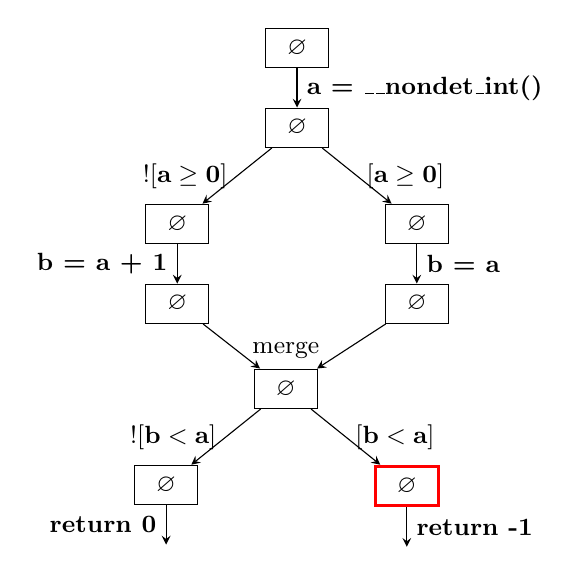
\begin{tikzpicture}[->,>=stealth, mynode/.style={rectangle, draw, minimum height=0.5cm, minimum width=0.8cm}, every node/.style={font=\small}]

  \node[mynode] (0) {$\varnothing$};
  \node[mynode] (1) [below = 0.5cm of 0]{$\varnothing$};
  \node[mynode] (2) [below left = 1cm of 1]{$\varnothing$};
  \node[mynode] (4) [below right = 1cm of 1]{$\varnothing$};
  \node[mynode] (3) [below = 0.5cm of 2]{$\varnothing$};
  \node[mynode] (5) [below = 0.5cm of 4]{$\varnothing$};
  \node[mynode] (6) [below right = 0.8cm of 3, label=north:merge]{$\varnothing$};
  \node[mynode] (7) [below left = 1cm of 6]{$\varnothing$};
  \node[mynode] (8) [below right = 1cm of 6, draw=red, very thick]{$\varnothing$};
  \coordinate[below = 0.5cm of 7] (e7);
  \coordinate[below = 0.5cm of 8] (e8);

  \path
    (0) edge node [right] {\textbf{a = \_\_nondet\_int()}} (1)
    (1) edge node [left, pos=0.5] {$\mathbf{![a \geq 0]}$} (2)
    (1) edge node [right, pos=0.5] {$\mathbf{[a \geq 0]}$} (4)
    (2) edge node [left] {\textbf{b = a + 1}} (3)
    (4) edge node [right] {\textbf{b = a}} (5)
    (3) edge (6)
    (5) edge (6)
    (6) edge node [left, pos=0.5] {$\mathbf{![b < a]}$} (7)
    (6) edge node [right, pos=0.5] {$\mathbf{[b < a]}$} (8)
    (7) edge node [left] {\textbf{return 0}} (e7)
    (8) edge node [right] {\textbf{return -1}} (e8)
  ;
\end{tikzpicture}
%\label{fig:ex1ValueGraph}
%\caption{Analysis of the program to the left by the \valueAnalysisCPA.}
\end{subfigure}
\caption{Simple program and its execution by the \valueAnalysisCPA.}
\label{fig:ex1}
\end{figure}

\begin{figure}[t]
\centering
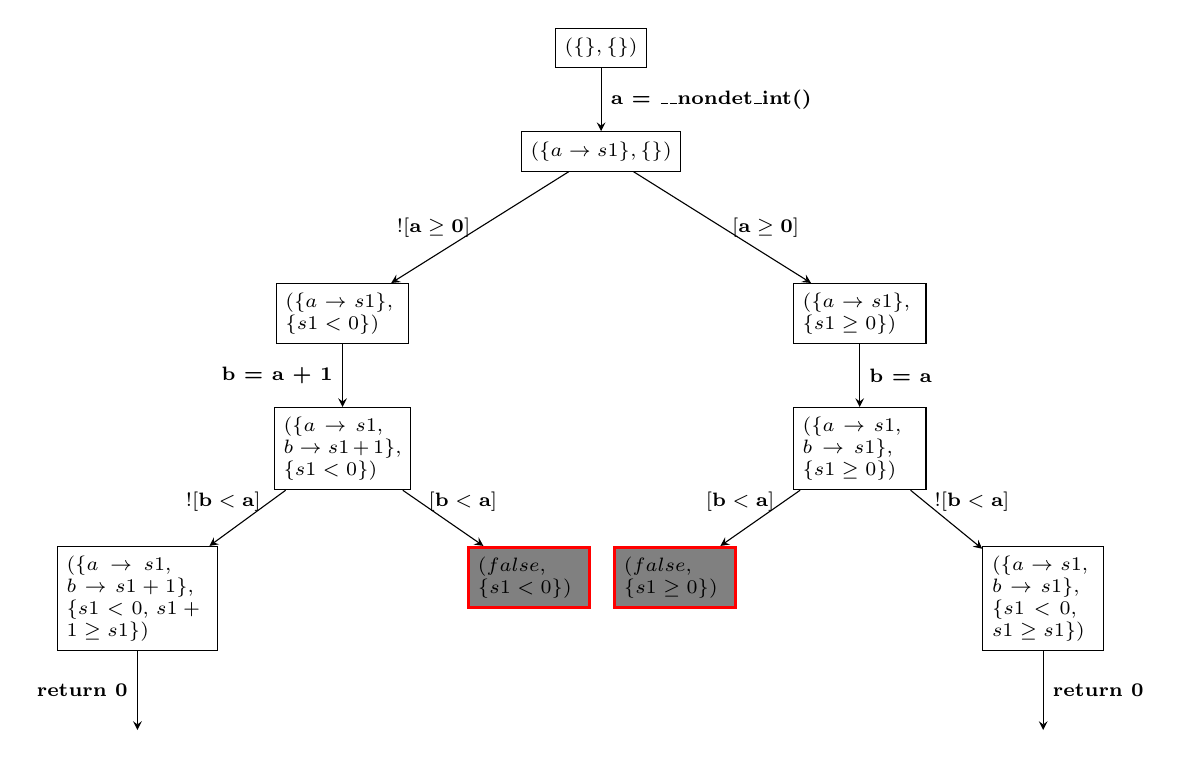
\begin{tikzpicture}[->,>=stealth, mynode/.style={rectangle, draw, minimum height=0.5cm, minimum width=0.8cm}, every node/.style={font=\scriptsize}]

  \node[mynode] (0) {$(\{\}, \{\})$};
  \node[mynode] (1) [below = 0.8cm of 0] {$(\{a \rightarrow s1\}, \{\})$};
  \node[mynode] (2) [below left = 2cm of 1, text width=1.45cm] {$(\{a \rightarrow s1\}$, $\{s1 < 0\})$};
  \node[mynode] (4) [below right = 2cm of 1, text width=1.45cm] {$(\{a \rightarrow s1\}$, $\{s1 \geq 0\})$};
  \node[mynode] (3) [below = 0.8cm of 2, text width=1.5cm] {$(\{a \rightarrow s1$, $b \rightarrow s1+1\}$, $\{s1 < 0\})$};
  \node[mynode] (5) [below = 0.8cm of 4, text width=1.45cm] {$(\{a \rightarrow s1$, $b \rightarrow s1 \}$, $\{s1 \geq 0\})$};
%  \node[mynode] (6) [below = 0.8cm of 3, text width=1.45cm] {$(\{a \rightarrow s1$, $b \rightarrow s1+1\}$, $\{s1 < 0\})$};
 % \node[mynode] (6n) [below = 0.8cm of 5, text width=1.45cm] {$(\{a \rightarrow s1$, $b \rightarrow s1 \}$, $\{s1 \geq 0\})$};
  \node[mynode] (7) [below left = 1cm of 3, text width=1.8cm] {$(\{a \rightarrow s1$, $b \rightarrow s1+1\}$, $\{s1 < 0$, $s1+1 \geq s1\})$};
  \node[mynode] (8) [below right = 1cm of 3, draw=red, fill=gray, very thick, text width=1.3cm]{$(false$, $\{s1 < 0\})$};
  \node[mynode] (8n) [below left = 1cm of 5, draw=red, fill=gray, very thick, text width=1.3cm]{$(false$, $\{s1 \geq 0\})$};
  \node[mynode] (7n) [below right = 1cm of 5, text width=1.3cm] {$(\{a \rightarrow s1$, $b \rightarrow s1\}$, $\{s1 < 0$, $s1 \geq s1\})$};
  \coordinate[below = 1cm of 7] (e7);
  \coordinate[below = 1cm of 7n] (e7n);

  \path
    (0) edge node [right] {\textbf{a = \_\_nondet\_int()}} (1)
    (1) edge node [left, pos=0.5] {$\mathbf{![a \geq 0]}$} (2)
    (1) edge node [right, pos=0.5] {$\mathbf{[a \geq 0]}$} (4)
    (2) edge node [left] {\textbf{b = a + 1}} (3)
    (4) edge node [right] {\textbf{b = a}} (5)
%    (3) edge (6)
%    (5) edge (6n)
    (3) edge node [left, pos=0.2] {$\mathbf{![b < a]}$} (7)
    (3) edge node [right, pos=0.2] {$\mathbf{[b < a]}$} (8)
    (5) edge node [left, pos=0.2] {$\mathbf{[b < a]}$} (8n)
    (5) edge node [right, pos=0.2] {$\mathbf{![b < a]}$} (7n)
    (7) edge node [left] {\textbf{return 0}} (e7)
    (7n) edge node [right] {\textbf{return 0}} (e7n)
  ;
\end{tikzpicture}
\caption{Analysis of the program in Listing \ref{lst:exProg} by the \symbolicExecutionCPA.}
\label{fig:ex1SymExGraph}
\end{figure}

%\subsubsection{Basic Value Analysis can't deal with non-deterministic values (+ Example)}
Figure \ref{fig:ex1} displays an example program that uses non-deterministic values and its analysis using the classic \valueAnalysisCPA.
Since the CPA does not store any information about non-deterministic assignments, no information about the relation between \textbf{a}\ and \textbf{b}\ exists and the property violation is reachable according to the analysis. This produces a \emph{false alarm}.
In constrast to this, the \symbolicExecutionCPA\ is able to handle the non-deterministic assignment to \textbf{a}\ a and its later usage. It returns that the program is safe, correctly.
Figure \ref{fig:ex1SymExGraph} shows this analysis. 

\SymbolicExecutionCPA's ability to track non-deterministic values is able to reduce the number of false alarms to a great extent, as we already showed in \cite{Lemberger2015}.
%\subsubsection{But symbolic value analysis pretty slow, as previous evaluation has shown (illustrate path explosion, sat checks)}
Runtime wise, it performs poorly, though, when compared to the \valueAnalysisCPA.
Since it considers all variable assignments, both deterministic and non-deterministic, and all occurring assumptions, its state space is exponential to the amount of occuring assumptions.
If a infinite loop occurs, the state space is infinite, too.
This problem is called \emph{path explosion}.\cite{Anand2008}
Obviously, an exponential amount of states does not scale to large programs.
In addition, the cost for SAT checks, which are performed at every assumption, are exponential to the amount of non-deterministic values occuring in all encountered assumptions on the currently considered program path.
Evaluation in \cite{Lemberger2015} showed that the \symbolicExecutionCPA\ spends up to 95\% of its runtime for SAT checks.

%\subsubsection{Goal: Try to speed up}
In this work we design, implement and evaluate different approaches to increasing the performance of the \symbolicExecutionCPA.
Our main contribution is, along with variations to the existing merge and less-or-equal operators of the CPA,
the application of CEGAR \cite{Clarke2003} to the composition of the two strongly intertwined CPAs \valueAnalysisCPA\ and \constraintsCPA\ with precision refinement for both CPAs
with two different precision types.

This work is divided into four parts: Theoretical background and contributions, their implementation, their evaluation, and future work and a conclusion.
First we will describe the concepts that are the basis for our work, such as Configurable Software Verification, used CPAs and CEGAR.
Next, we will illustrate the theory behind our own contribution,
before explaining details about the existing and newly added implementation and deviations from theory.
We will evaluate all presented concepts and compare them to the performance of the \valueAnalysisCPA, \predicateCPA, and \symbolicExecutionCPA\ of our old work.
Last, we will give a short outlook to possible future work in this field and close with a conclusion.
%%%%%%%%%%%%%%%%%%%%%%%%%%%%%%%%
\section{Introduction}
%\subsubsection{Why Software Verification is important/needed}
Software systems are prone to error due to multiple factors: The developers skills, humans' limited understanding of software principles, communication problems in development, missing or sparse documentation and unforeseen interdependencies between software components are just some of them.

Because of this testing has been an integral part of software development for quite some time, often claiming about 50\% of development effort and more than 50\% of the budget.
\emph{Software testing} describes the execution of a program with the intention of finding errors.
The tester, either a person or another program, uses different inputs and checks that the proper output is produced.
The nature of this approach determines that only a finite amount of inputs is possible in finite time.
As a result, it is impossible to ensure the errorless execution of a program with arbitrary input.
Additionally, human testing is a technique only shortly touched in most software engineering educations, resembling art more than science.\cite{Myers2011}

Along with these points, the rise of ubiquitious computing and reactive systems complicates the process of reliable verification by testing even more.
Always running systems that gather, evaluate and adapt their behaviour to information of their environment pose an immense amount of possible inputs and interactions due to these.
This makes it almost impossible to predict the behaviour of such systems through testing.

An alternative to testing is formal verification, which tries to produce formal statements that are true for all possible behaviours of a system, using mathematical methods.
These statements are then used for proving that a specific specification is met.
One area of formal verification is \emph{automated software verification}. It tries to reach the above goal by only using software that works without the help or feedback of humans.
\CpaChecker\ \cite{Beyer2011} is such a program that yielded excellent performance in the last iterations of  the \href{http://sv-comp.sosy-lab.org}{Competition on Software Verification} (SV-COMP) \cite{SV-COMP2013} \cite{SV-COMP2014} \cite{SV-COMP2015}.
\CpaChecker\ is a framework for \emph{Configurable Software Verification} \cite{Beyer2007} utilizing different \emph{configurable program analyses} (CPAs) to locate possible property violations of a specification in a program.
Three such CPAs are the \valueAnalysisCPA, which uses concrete variable assignments, the \predicateCPA, which creates predicates for describing properties of program paths,
and the \symbolicExecutionCPA, which uses an extension of the \valueAnalysisCPA\ tracking non-deterministic values as symbolic ones in combination with the \constraintsCPA, which tracks constraints to symbolic values on program paths.
While the \valueAnalysisCPA\ has high efficiency due to her simplicity, it can't handle complex program characteristics like pointers or non-deterministic values.
The \predicateCPA, in constrast, is very expressive, but has low efficiency since SAT checks are necessary for computing the feasibility of a program path.
The \symbolicExecutionCPA\ poses something in between those two, not being able to handle some complex program characteristics as it is partly based on the \valueAnalysisCPA, but being able to handle non-deterministic values.
On the other hand, it uses SAT checks, too, though less often and over smaller formulas.

\begin{figure}[t]
\lstset{numbers=left}
\begin{subfigure}[b]{.45\textwidth}
\lstinputlisting[language=C]{exampleProgram.c}
%\caption{A simple non-deterministic program.}
%\label{lst:exProg}
\end{subfigure}%
\hfill
\begin{subfigure}[b]{.45\textwidth}
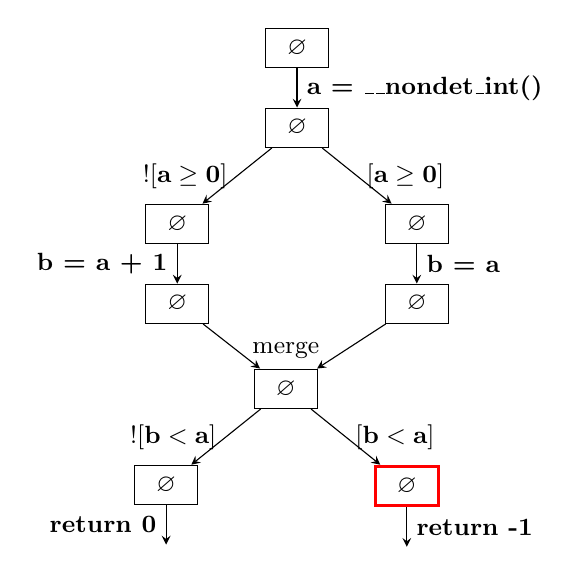
\begin{tikzpicture}[->,>=stealth, mynode/.style={rectangle, draw, minimum height=0.5cm, minimum width=0.8cm}, every node/.style={font=\small}]

  \node[mynode] (0) {$\varnothing$};
  \node[mynode] (1) [below = 0.5cm of 0]{$\varnothing$};
  \node[mynode] (2) [below left = 1cm of 1]{$\varnothing$};
  \node[mynode] (4) [below right = 1cm of 1]{$\varnothing$};
  \node[mynode] (3) [below = 0.5cm of 2]{$\varnothing$};
  \node[mynode] (5) [below = 0.5cm of 4]{$\varnothing$};
  \node[mynode] (6) [below right = 0.8cm of 3, label=north:merge]{$\varnothing$};
  \node[mynode] (7) [below left = 1cm of 6]{$\varnothing$};
  \node[mynode] (8) [below right = 1cm of 6, draw=red, very thick]{$\varnothing$};
  \coordinate[below = 0.5cm of 7] (e7);
  \coordinate[below = 0.5cm of 8] (e8);

  \path
    (0) edge node [right] {\textbf{a = \_\_nondet\_int()}} (1)
    (1) edge node [left, pos=0.5] {$\mathbf{![a \geq 0]}$} (2)
    (1) edge node [right, pos=0.5] {$\mathbf{[a \geq 0]}$} (4)
    (2) edge node [left] {\textbf{b = a + 1}} (3)
    (4) edge node [right] {\textbf{b = a}} (5)
    (3) edge (6)
    (5) edge (6)
    (6) edge node [left, pos=0.5] {$\mathbf{![b < a]}$} (7)
    (6) edge node [right, pos=0.5] {$\mathbf{[b < a]}$} (8)
    (7) edge node [left] {\textbf{return 0}} (e7)
    (8) edge node [right] {\textbf{return -1}} (e8)
  ;
\end{tikzpicture}
%\label{fig:ex1ValueGraph}
%\caption{Analysis of the program to the left by the \valueAnalysisCPA.}
\end{subfigure}
\caption{Simple program and its execution by the \valueAnalysisCPA.}
\label{fig:ex1}
\end{figure}

\begin{figure}[t]
\centering
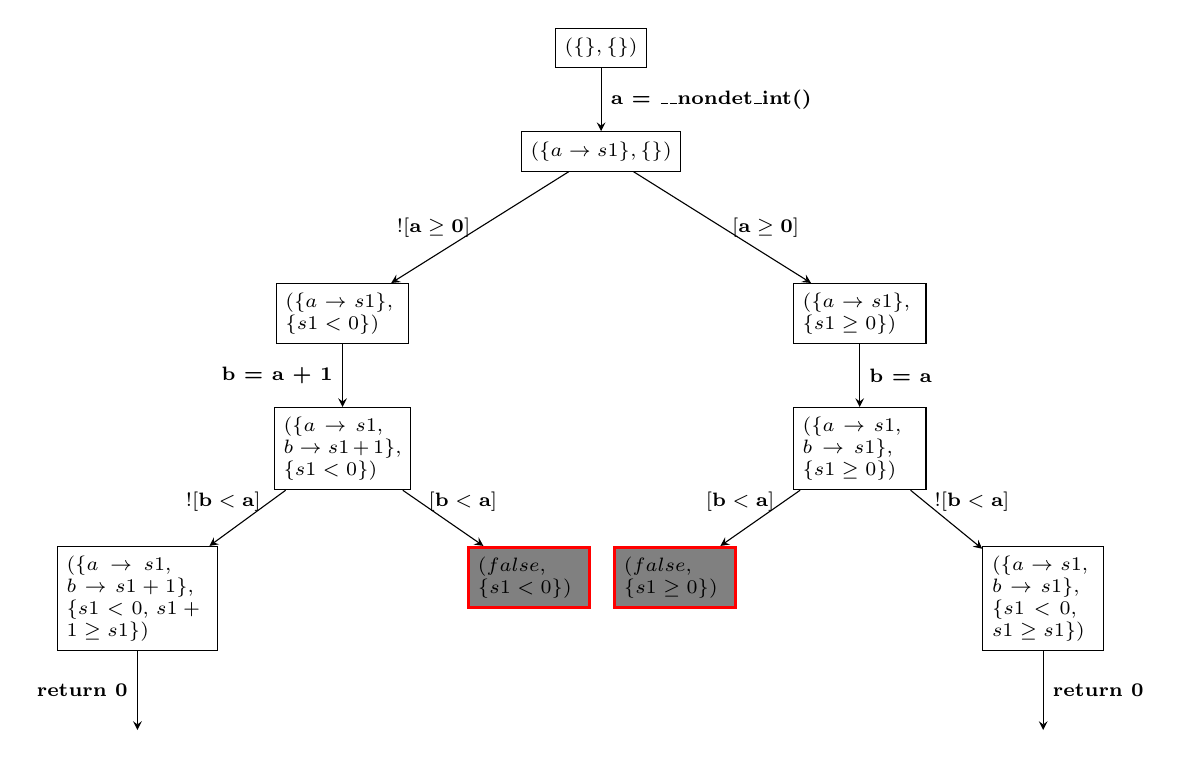
\begin{tikzpicture}[->,>=stealth, mynode/.style={rectangle, draw, minimum height=0.5cm, minimum width=0.8cm}, every node/.style={font=\scriptsize}]

  \node[mynode] (0) {$(\{\}, \{\})$};
  \node[mynode] (1) [below = 0.8cm of 0] {$(\{a \rightarrow s1\}, \{\})$};
  \node[mynode] (2) [below left = 2cm of 1, text width=1.45cm] {$(\{a \rightarrow s1\}$, $\{s1 < 0\})$};
  \node[mynode] (4) [below right = 2cm of 1, text width=1.45cm] {$(\{a \rightarrow s1\}$, $\{s1 \geq 0\})$};
  \node[mynode] (3) [below = 0.8cm of 2, text width=1.5cm] {$(\{a \rightarrow s1$, $b \rightarrow s1+1\}$, $\{s1 < 0\})$};
  \node[mynode] (5) [below = 0.8cm of 4, text width=1.45cm] {$(\{a \rightarrow s1$, $b \rightarrow s1 \}$, $\{s1 \geq 0\})$};
%  \node[mynode] (6) [below = 0.8cm of 3, text width=1.45cm] {$(\{a \rightarrow s1$, $b \rightarrow s1+1\}$, $\{s1 < 0\})$};
 % \node[mynode] (6n) [below = 0.8cm of 5, text width=1.45cm] {$(\{a \rightarrow s1$, $b \rightarrow s1 \}$, $\{s1 \geq 0\})$};
  \node[mynode] (7) [below left = 1cm of 3, text width=1.8cm] {$(\{a \rightarrow s1$, $b \rightarrow s1+1\}$, $\{s1 < 0$, $s1+1 \geq s1\})$};
  \node[mynode] (8) [below right = 1cm of 3, draw=red, fill=gray, very thick, text width=1.3cm]{$(false$, $\{s1 < 0\})$};
  \node[mynode] (8n) [below left = 1cm of 5, draw=red, fill=gray, very thick, text width=1.3cm]{$(false$, $\{s1 \geq 0\})$};
  \node[mynode] (7n) [below right = 1cm of 5, text width=1.3cm] {$(\{a \rightarrow s1$, $b \rightarrow s1\}$, $\{s1 < 0$, $s1 \geq s1\})$};
  \coordinate[below = 1cm of 7] (e7);
  \coordinate[below = 1cm of 7n] (e7n);

  \path
    (0) edge node [right] {\textbf{a = \_\_nondet\_int()}} (1)
    (1) edge node [left, pos=0.5] {$\mathbf{![a \geq 0]}$} (2)
    (1) edge node [right, pos=0.5] {$\mathbf{[a \geq 0]}$} (4)
    (2) edge node [left] {\textbf{b = a + 1}} (3)
    (4) edge node [right] {\textbf{b = a}} (5)
%    (3) edge (6)
%    (5) edge (6n)
    (3) edge node [left, pos=0.2] {$\mathbf{![b < a]}$} (7)
    (3) edge node [right, pos=0.2] {$\mathbf{[b < a]}$} (8)
    (5) edge node [left, pos=0.2] {$\mathbf{[b < a]}$} (8n)
    (5) edge node [right, pos=0.2] {$\mathbf{![b < a]}$} (7n)
    (7) edge node [left] {\textbf{return 0}} (e7)
    (7n) edge node [right] {\textbf{return 0}} (e7n)
  ;
\end{tikzpicture}
\caption{Analysis of the program in Listing \ref{lst:exProg} by the \symbolicExecutionCPA.}
\label{fig:ex1SymExGraph}
\end{figure}

%\subsubsection{Basic Value Analysis can't deal with non-deterministic values (+ Example)}
Figure \ref{fig:ex1} displays an example program that uses non-deterministic values and its analysis using the classic \valueAnalysisCPA.
Since the CPA does not store any information about non-deterministic assignments, no information about the relation between \textbf{a}\ and \textbf{b}\ exists and the property violation is reachable according to the analysis. This produces a \emph{false alarm}.
In constrast to this, the \symbolicExecutionCPA\ is able to handle the non-deterministic assignment to \textbf{a}\ a and its later usage. It returns that the program is safe, correctly.
Figure \ref{fig:ex1SymExGraph} shows this analysis. 

\SymbolicExecutionCPA's ability to track non-deterministic values is able to reduce the number of false alarms to a great extent, as we already showed in \cite{Lemberger2015}.
%\subsubsection{But symbolic value analysis pretty slow, as previous evaluation has shown (illustrate path explosion, sat checks)}
Runtime wise, it performs poorly, though, when compared to the \valueAnalysisCPA.
Since it considers all variable assignments, both deterministic and non-deterministic, and all occurring assumptions, its state space is exponential to the amount of occuring assumptions.
If a infinite loop occurs, the state space is infinite, too.
This problem is called \emph{path explosion}.\cite{Anand2008}
Obviously, an exponential amount of states does not scale to large programs.
In addition, the cost for SAT checks, which are performed at every assumption, are exponential to the amount of non-deterministic values occuring in all encountered assumptions on the currently considered program path.
Evaluation in \cite{Lemberger2015} showed that the \symbolicExecutionCPA\ spends up to 95\% of its runtime for SAT checks.

%\subsubsection{Goal: Try to speed up}
In this work we design, implement and evaluate different approaches to increasing the performance of the \symbolicExecutionCPA.
Our main contribution is, along with variations to the existing merge and less-or-equal operators of the CPA,
the application of CEGAR \cite{Clarke2003} to the composition of the two strongly intertwined CPAs \valueAnalysisCPA\ and \constraintsCPA\ with precision refinement for both CPAs
with two different precision types.

This work is divided into four parts: Theoretical background and contributions, their implementation, their evaluation, and future work and a conclusion.
First we will describe the concepts that are the basis for our work, such as Configurable Software Verification, used CPAs and CEGAR.
Next, we will illustrate the theory behind our own contribution,
before explaining details about the existing and newly added implementation and deviations from theory.
We will evaluate all presented concepts and compare them to the performance of the \valueAnalysisCPA, \predicateCPA, and \symbolicExecutionCPA\ of our old work.
Last, we will give a short outlook to possible future work in this field and close with a conclusion.
%%%%%%%%%%%%%%%%%%%%%%%%%%%%%%%%
\section{Introduction}
%\subsubsection{Why Software Verification is important/needed}
Software systems are prone to error due to multiple factors: The developers skills, humans' limited understanding of software principles, communication problems in development, missing or sparse documentation and unforeseen interdependencies between software components are just some of them.

Because of this testing has been an integral part of software development for quite some time, often claiming about 50\% of development effort and more than 50\% of the budget.
\emph{Software testing} describes the execution of a program with the intention of finding errors.
The tester, either a person or another program, uses different inputs and checks that the proper output is produced.
The nature of this approach determines that only a finite amount of inputs is possible in finite time.
As a result, it is impossible to ensure the errorless execution of a program with arbitrary input.
Additionally, human testing is a technique only shortly touched in most software engineering educations, resembling art more than science.\cite{Myers2011}

Along with these points, the rise of ubiquitious computing and reactive systems complicates the process of reliable verification by testing even more.
Always running systems that gather, evaluate and adapt their behaviour to information of their environment pose an immense amount of possible inputs and interactions due to these.
This makes it almost impossible to predict the behaviour of such systems through testing.

An alternative to testing is formal verification, which tries to produce formal statements that are true for all possible behaviours of a system, using mathematical methods.
These statements are then used for proving that a specific specification is met.
One area of formal verification is \emph{automated software verification}. It tries to reach the above goal by only using software that works without the help or feedback of humans.
\CpaChecker\ \cite{Beyer2011} is such a program that yielded excellent performance in the last iterations of  the \href{http://sv-comp.sosy-lab.org}{Competition on Software Verification} (SV-COMP) \cite{SV-COMP2013} \cite{SV-COMP2014} \cite{SV-COMP2015}.
\CpaChecker\ is a framework for \emph{Configurable Software Verification} \cite{Beyer2007} utilizing different \emph{configurable program analyses} (CPAs) to locate possible property violations of a specification in a program.
Three such CPAs are the \valueAnalysisCPA, which uses concrete variable assignments, the \predicateCPA, which creates predicates for describing properties of program paths,
and the \symbolicExecutionCPA, which uses an extension of the \valueAnalysisCPA\ tracking non-deterministic values as symbolic ones in combination with the \constraintsCPA, which tracks constraints to symbolic values on program paths.
While the \valueAnalysisCPA\ has high efficiency due to her simplicity, it can't handle complex program characteristics like pointers or non-deterministic values.
The \predicateCPA, in constrast, is very expressive, but has low efficiency since SAT checks are necessary for computing the feasibility of a program path.
The \symbolicExecutionCPA\ poses something in between those two, not being able to handle some complex program characteristics as it is partly based on the \valueAnalysisCPA, but being able to handle non-deterministic values.
On the other hand, it uses SAT checks, too, though less often and over smaller formulas.

\begin{figure}[t]
\lstset{numbers=left}
\begin{subfigure}[b]{.45\textwidth}
\lstinputlisting[language=C]{exampleProgram.c}
%\caption{A simple non-deterministic program.}
%\label{lst:exProg}
\end{subfigure}%
\hfill
\begin{subfigure}[b]{.45\textwidth}
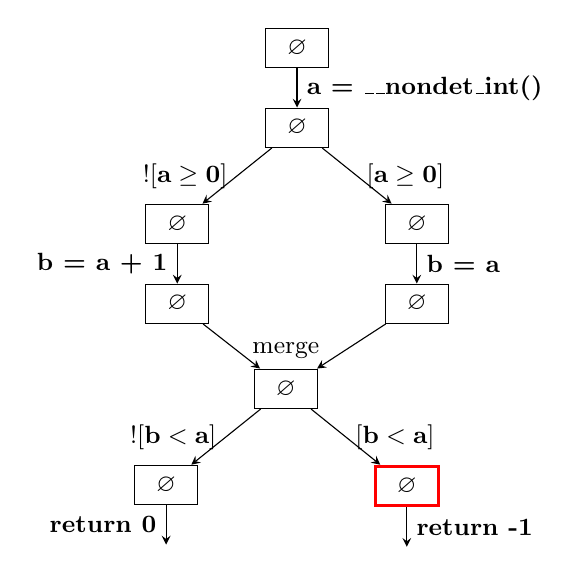
\begin{tikzpicture}[->,>=stealth, mynode/.style={rectangle, draw, minimum height=0.5cm, minimum width=0.8cm}, every node/.style={font=\small}]

  \node[mynode] (0) {$\varnothing$};
  \node[mynode] (1) [below = 0.5cm of 0]{$\varnothing$};
  \node[mynode] (2) [below left = 1cm of 1]{$\varnothing$};
  \node[mynode] (4) [below right = 1cm of 1]{$\varnothing$};
  \node[mynode] (3) [below = 0.5cm of 2]{$\varnothing$};
  \node[mynode] (5) [below = 0.5cm of 4]{$\varnothing$};
  \node[mynode] (6) [below right = 0.8cm of 3, label=north:merge]{$\varnothing$};
  \node[mynode] (7) [below left = 1cm of 6]{$\varnothing$};
  \node[mynode] (8) [below right = 1cm of 6, draw=red, very thick]{$\varnothing$};
  \coordinate[below = 0.5cm of 7] (e7);
  \coordinate[below = 0.5cm of 8] (e8);

  \path
    (0) edge node [right] {\textbf{a = \_\_nondet\_int()}} (1)
    (1) edge node [left, pos=0.5] {$\mathbf{![a \geq 0]}$} (2)
    (1) edge node [right, pos=0.5] {$\mathbf{[a \geq 0]}$} (4)
    (2) edge node [left] {\textbf{b = a + 1}} (3)
    (4) edge node [right] {\textbf{b = a}} (5)
    (3) edge (6)
    (5) edge (6)
    (6) edge node [left, pos=0.5] {$\mathbf{![b < a]}$} (7)
    (6) edge node [right, pos=0.5] {$\mathbf{[b < a]}$} (8)
    (7) edge node [left] {\textbf{return 0}} (e7)
    (8) edge node [right] {\textbf{return -1}} (e8)
  ;
\end{tikzpicture}
%\label{fig:ex1ValueGraph}
%\caption{Analysis of the program to the left by the \valueAnalysisCPA.}
\end{subfigure}
\caption{Simple program and its execution by the \valueAnalysisCPA.}
\label{fig:ex1}
\end{figure}

\begin{figure}[t]
\centering
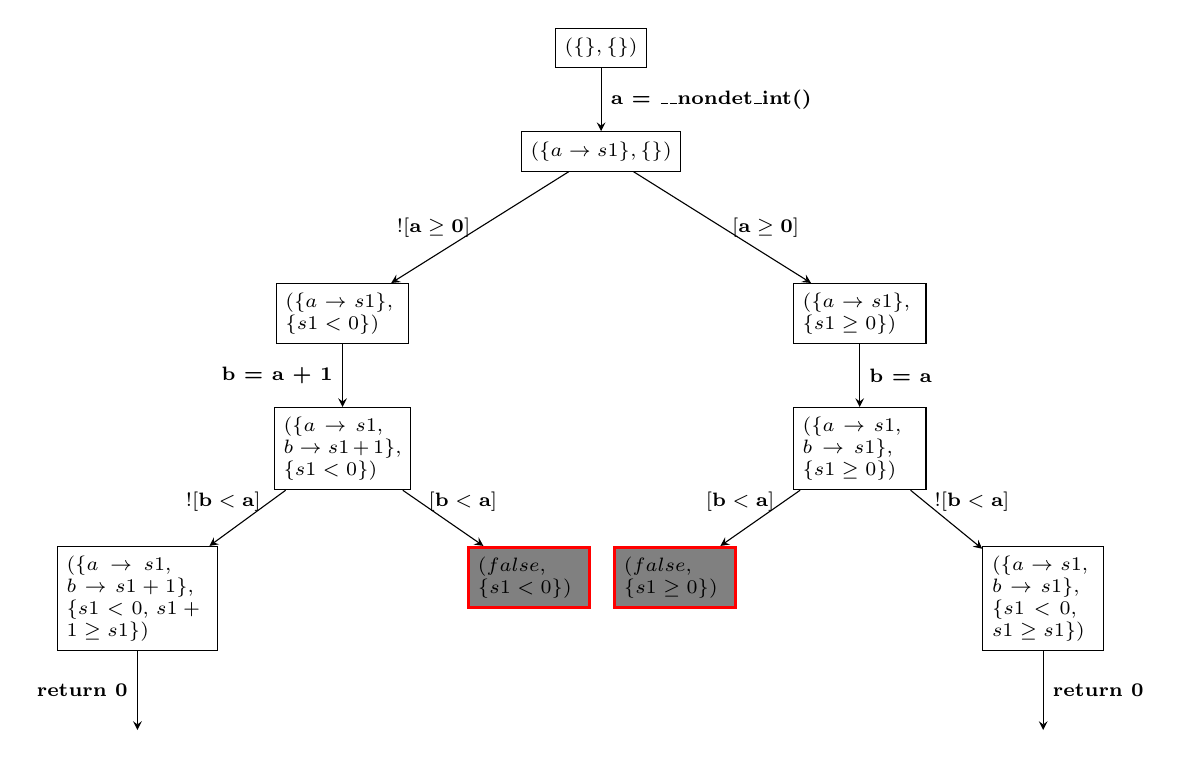
\begin{tikzpicture}[->,>=stealth, mynode/.style={rectangle, draw, minimum height=0.5cm, minimum width=0.8cm}, every node/.style={font=\scriptsize}]

  \node[mynode] (0) {$(\{\}, \{\})$};
  \node[mynode] (1) [below = 0.8cm of 0] {$(\{a \rightarrow s1\}, \{\})$};
  \node[mynode] (2) [below left = 2cm of 1, text width=1.45cm] {$(\{a \rightarrow s1\}$, $\{s1 < 0\})$};
  \node[mynode] (4) [below right = 2cm of 1, text width=1.45cm] {$(\{a \rightarrow s1\}$, $\{s1 \geq 0\})$};
  \node[mynode] (3) [below = 0.8cm of 2, text width=1.5cm] {$(\{a \rightarrow s1$, $b \rightarrow s1+1\}$, $\{s1 < 0\})$};
  \node[mynode] (5) [below = 0.8cm of 4, text width=1.45cm] {$(\{a \rightarrow s1$, $b \rightarrow s1 \}$, $\{s1 \geq 0\})$};
%  \node[mynode] (6) [below = 0.8cm of 3, text width=1.45cm] {$(\{a \rightarrow s1$, $b \rightarrow s1+1\}$, $\{s1 < 0\})$};
 % \node[mynode] (6n) [below = 0.8cm of 5, text width=1.45cm] {$(\{a \rightarrow s1$, $b \rightarrow s1 \}$, $\{s1 \geq 0\})$};
  \node[mynode] (7) [below left = 1cm of 3, text width=1.8cm] {$(\{a \rightarrow s1$, $b \rightarrow s1+1\}$, $\{s1 < 0$, $s1+1 \geq s1\})$};
  \node[mynode] (8) [below right = 1cm of 3, draw=red, fill=gray, very thick, text width=1.3cm]{$(false$, $\{s1 < 0\})$};
  \node[mynode] (8n) [below left = 1cm of 5, draw=red, fill=gray, very thick, text width=1.3cm]{$(false$, $\{s1 \geq 0\})$};
  \node[mynode] (7n) [below right = 1cm of 5, text width=1.3cm] {$(\{a \rightarrow s1$, $b \rightarrow s1\}$, $\{s1 < 0$, $s1 \geq s1\})$};
  \coordinate[below = 1cm of 7] (e7);
  \coordinate[below = 1cm of 7n] (e7n);

  \path
    (0) edge node [right] {\textbf{a = \_\_nondet\_int()}} (1)
    (1) edge node [left, pos=0.5] {$\mathbf{![a \geq 0]}$} (2)
    (1) edge node [right, pos=0.5] {$\mathbf{[a \geq 0]}$} (4)
    (2) edge node [left] {\textbf{b = a + 1}} (3)
    (4) edge node [right] {\textbf{b = a}} (5)
%    (3) edge (6)
%    (5) edge (6n)
    (3) edge node [left, pos=0.2] {$\mathbf{![b < a]}$} (7)
    (3) edge node [right, pos=0.2] {$\mathbf{[b < a]}$} (8)
    (5) edge node [left, pos=0.2] {$\mathbf{[b < a]}$} (8n)
    (5) edge node [right, pos=0.2] {$\mathbf{![b < a]}$} (7n)
    (7) edge node [left] {\textbf{return 0}} (e7)
    (7n) edge node [right] {\textbf{return 0}} (e7n)
  ;
\end{tikzpicture}
\caption{Analysis of the program in Listing \ref{lst:exProg} by the \symbolicExecutionCPA.}
\label{fig:ex1SymExGraph}
\end{figure}

%\subsubsection{Basic Value Analysis can't deal with non-deterministic values (+ Example)}
Figure \ref{fig:ex1} displays an example program that uses non-deterministic values and its analysis using the classic \valueAnalysisCPA.
Since the CPA does not store any information about non-deterministic assignments, no information about the relation between \textbf{a}\ and \textbf{b}\ exists and the property violation is reachable according to the analysis. This produces a \emph{false alarm}.
In constrast to this, the \symbolicExecutionCPA\ is able to handle the non-deterministic assignment to \textbf{a}\ a and its later usage. It returns that the program is safe, correctly.
Figure \ref{fig:ex1SymExGraph} shows this analysis. 

\SymbolicExecutionCPA's ability to track non-deterministic values is able to reduce the number of false alarms to a great extent, as we already showed in \cite{Lemberger2015}.
%\subsubsection{But symbolic value analysis pretty slow, as previous evaluation has shown (illustrate path explosion, sat checks)}
Runtime wise, it performs poorly, though, when compared to the \valueAnalysisCPA.
Since it considers all variable assignments, both deterministic and non-deterministic, and all occurring assumptions, its state space is exponential to the amount of occuring assumptions.
If a infinite loop occurs, the state space is infinite, too.
This problem is called \emph{path explosion}.\cite{Anand2008}
Obviously, an exponential amount of states does not scale to large programs.
In addition, the cost for SAT checks, which are performed at every assumption, are exponential to the amount of non-deterministic values occuring in all encountered assumptions on the currently considered program path.
Evaluation in \cite{Lemberger2015} showed that the \symbolicExecutionCPA\ spends up to 95\% of its runtime for SAT checks.

%\subsubsection{Goal: Try to speed up}
In this work we design, implement and evaluate different approaches to increasing the performance of the \symbolicExecutionCPA.
Our main contribution is, along with variations to the existing merge and less-or-equal operators of the CPA,
the application of CEGAR \cite{Clarke2003} to the composition of the two strongly intertwined CPAs \valueAnalysisCPA\ and \constraintsCPA\ with precision refinement for both CPAs
with two different precision types.

This work is divided into four parts: Theoretical background and contributions, their implementation, their evaluation, and future work and a conclusion.
First we will describe the concepts that are the basis for our work, such as Configurable Software Verification, used CPAs and CEGAR.
Next, we will illustrate the theory behind our own contribution,
before explaining details about the existing and newly added implementation and deviations from theory.
We will evaluate all presented concepts and compare them to the performance of the \valueAnalysisCPA, \predicateCPA, and \symbolicExecutionCPA\ of our old work.
Last, we will give a short outlook to possible future work in this field and close with a conclusion.
%%%%%%%%%%%%%%%%%%%%%%%%%%%%%%%%
\section{Introduction}
%\subsubsection{Why Software Verification is important/needed}
Software systems are prone to error due to multiple factors: The developers skills, humans' limited understanding of software principles, communication problems in development, missing or sparse documentation and unforeseen interdependencies between software components are just some of them.

Because of this testing has been an integral part of software development for quite some time, often claiming about 50\% of development effort and more than 50\% of the budget.
\emph{Software testing} describes the execution of a program with the intention of finding errors.
The tester, either a person or another program, uses different inputs and checks that the proper output is produced.
The nature of this approach determines that only a finite amount of inputs is possible in finite time.
As a result, it is impossible to ensure the errorless execution of a program with arbitrary input.
Additionally, human testing is a technique only shortly touched in most software engineering educations, resembling art more than science.\cite{Myers2011}

Along with these points, the rise of ubiquitious computing and reactive systems complicates the process of reliable verification by testing even more.
Always running systems that gather, evaluate and adapt their behaviour to information of their environment pose an immense amount of possible inputs and interactions due to these.
This makes it almost impossible to predict the behaviour of such systems through testing.

An alternative to testing is formal verification, which tries to produce formal statements that are true for all possible behaviours of a system, using mathematical methods.
These statements are then used for proving that a specific specification is met.
One area of formal verification is \emph{automated software verification}. It tries to reach the above goal by only using software that works without the help or feedback of humans.
\CpaChecker\ \cite{Beyer2011} is such a program that yielded excellent performance in the last iterations of  the \href{http://sv-comp.sosy-lab.org}{Competition on Software Verification} (SV-COMP) \cite{SV-COMP2013} \cite{SV-COMP2014} \cite{SV-COMP2015}.
\CpaChecker\ is a framework for \emph{Configurable Software Verification} \cite{Beyer2007} utilizing different \emph{configurable program analyses} (CPAs) to locate possible property violations of a specification in a program.
Three such CPAs are the \valueAnalysisCPA, which uses concrete variable assignments, the \predicateCPA, which creates predicates for describing properties of program paths,
and the \symbolicExecutionCPA, which uses an extension of the \valueAnalysisCPA\ tracking non-deterministic values as symbolic ones in combination with the \constraintsCPA, which tracks constraints to symbolic values on program paths.
While the \valueAnalysisCPA\ has high efficiency due to her simplicity, it can't handle complex program characteristics like pointers or non-deterministic values.
The \predicateCPA, in constrast, is very expressive, but has low efficiency since SAT checks are necessary for computing the feasibility of a program path.
The \symbolicExecutionCPA\ poses something in between those two, not being able to handle some complex program characteristics as it is partly based on the \valueAnalysisCPA, but being able to handle non-deterministic values.
On the other hand, it uses SAT checks, too, though less often and over smaller formulas.

\begin{figure}[t]
\lstset{numbers=left}
\begin{subfigure}[b]{.45\textwidth}
\lstinputlisting[language=C]{exampleProgram.c}
%\caption{A simple non-deterministic program.}
%\label{lst:exProg}
\end{subfigure}%
\hfill
\begin{subfigure}[b]{.45\textwidth}
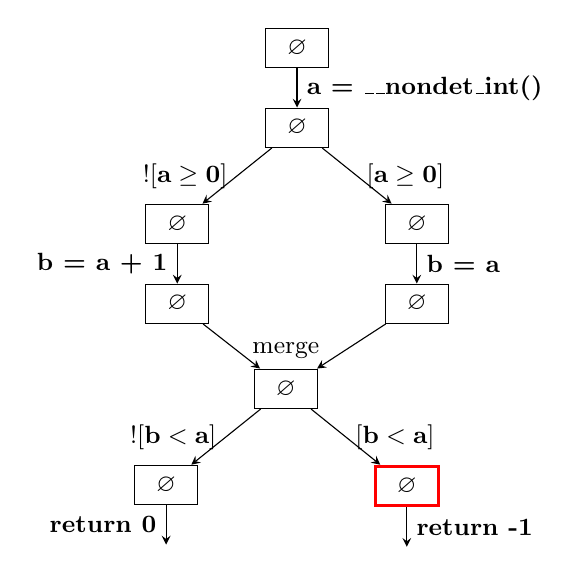
\begin{tikzpicture}[->,>=stealth, mynode/.style={rectangle, draw, minimum height=0.5cm, minimum width=0.8cm}, every node/.style={font=\small}]

  \node[mynode] (0) {$\varnothing$};
  \node[mynode] (1) [below = 0.5cm of 0]{$\varnothing$};
  \node[mynode] (2) [below left = 1cm of 1]{$\varnothing$};
  \node[mynode] (4) [below right = 1cm of 1]{$\varnothing$};
  \node[mynode] (3) [below = 0.5cm of 2]{$\varnothing$};
  \node[mynode] (5) [below = 0.5cm of 4]{$\varnothing$};
  \node[mynode] (6) [below right = 0.8cm of 3, label=north:merge]{$\varnothing$};
  \node[mynode] (7) [below left = 1cm of 6]{$\varnothing$};
  \node[mynode] (8) [below right = 1cm of 6, draw=red, very thick]{$\varnothing$};
  \coordinate[below = 0.5cm of 7] (e7);
  \coordinate[below = 0.5cm of 8] (e8);

  \path
    (0) edge node [right] {\textbf{a = \_\_nondet\_int()}} (1)
    (1) edge node [left, pos=0.5] {$\mathbf{![a \geq 0]}$} (2)
    (1) edge node [right, pos=0.5] {$\mathbf{[a \geq 0]}$} (4)
    (2) edge node [left] {\textbf{b = a + 1}} (3)
    (4) edge node [right] {\textbf{b = a}} (5)
    (3) edge (6)
    (5) edge (6)
    (6) edge node [left, pos=0.5] {$\mathbf{![b < a]}$} (7)
    (6) edge node [right, pos=0.5] {$\mathbf{[b < a]}$} (8)
    (7) edge node [left] {\textbf{return 0}} (e7)
    (8) edge node [right] {\textbf{return -1}} (e8)
  ;
\end{tikzpicture}
%\label{fig:ex1ValueGraph}
%\caption{Analysis of the program to the left by the \valueAnalysisCPA.}
\end{subfigure}
\caption{Simple program and its execution by the \valueAnalysisCPA.}
\label{fig:ex1}
\end{figure}

\begin{figure}[t]
\centering
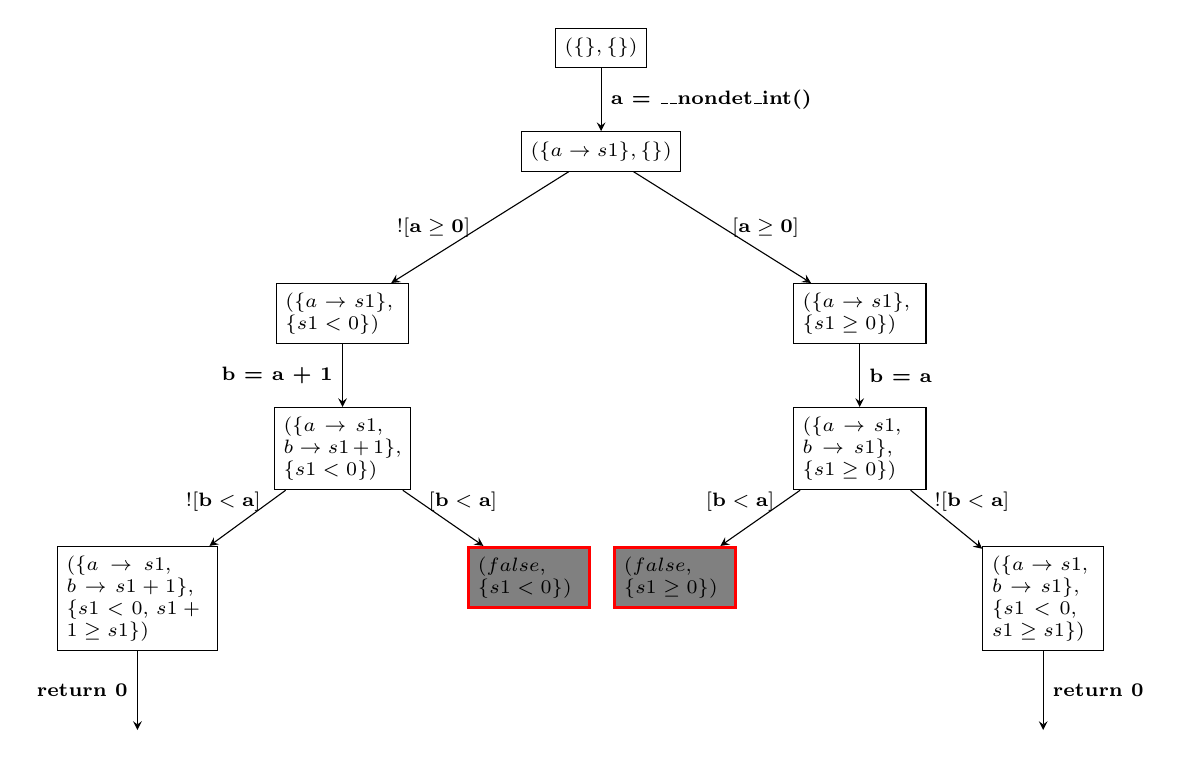
\begin{tikzpicture}[->,>=stealth, mynode/.style={rectangle, draw, minimum height=0.5cm, minimum width=0.8cm}, every node/.style={font=\scriptsize}]

  \node[mynode] (0) {$(\{\}, \{\})$};
  \node[mynode] (1) [below = 0.8cm of 0] {$(\{a \rightarrow s1\}, \{\})$};
  \node[mynode] (2) [below left = 2cm of 1, text width=1.45cm] {$(\{a \rightarrow s1\}$, $\{s1 < 0\})$};
  \node[mynode] (4) [below right = 2cm of 1, text width=1.45cm] {$(\{a \rightarrow s1\}$, $\{s1 \geq 0\})$};
  \node[mynode] (3) [below = 0.8cm of 2, text width=1.5cm] {$(\{a \rightarrow s1$, $b \rightarrow s1+1\}$, $\{s1 < 0\})$};
  \node[mynode] (5) [below = 0.8cm of 4, text width=1.45cm] {$(\{a \rightarrow s1$, $b \rightarrow s1 \}$, $\{s1 \geq 0\})$};
%  \node[mynode] (6) [below = 0.8cm of 3, text width=1.45cm] {$(\{a \rightarrow s1$, $b \rightarrow s1+1\}$, $\{s1 < 0\})$};
 % \node[mynode] (6n) [below = 0.8cm of 5, text width=1.45cm] {$(\{a \rightarrow s1$, $b \rightarrow s1 \}$, $\{s1 \geq 0\})$};
  \node[mynode] (7) [below left = 1cm of 3, text width=1.8cm] {$(\{a \rightarrow s1$, $b \rightarrow s1+1\}$, $\{s1 < 0$, $s1+1 \geq s1\})$};
  \node[mynode] (8) [below right = 1cm of 3, draw=red, fill=gray, very thick, text width=1.3cm]{$(false$, $\{s1 < 0\})$};
  \node[mynode] (8n) [below left = 1cm of 5, draw=red, fill=gray, very thick, text width=1.3cm]{$(false$, $\{s1 \geq 0\})$};
  \node[mynode] (7n) [below right = 1cm of 5, text width=1.3cm] {$(\{a \rightarrow s1$, $b \rightarrow s1\}$, $\{s1 < 0$, $s1 \geq s1\})$};
  \coordinate[below = 1cm of 7] (e7);
  \coordinate[below = 1cm of 7n] (e7n);

  \path
    (0) edge node [right] {\textbf{a = \_\_nondet\_int()}} (1)
    (1) edge node [left, pos=0.5] {$\mathbf{![a \geq 0]}$} (2)
    (1) edge node [right, pos=0.5] {$\mathbf{[a \geq 0]}$} (4)
    (2) edge node [left] {\textbf{b = a + 1}} (3)
    (4) edge node [right] {\textbf{b = a}} (5)
%    (3) edge (6)
%    (5) edge (6n)
    (3) edge node [left, pos=0.2] {$\mathbf{![b < a]}$} (7)
    (3) edge node [right, pos=0.2] {$\mathbf{[b < a]}$} (8)
    (5) edge node [left, pos=0.2] {$\mathbf{[b < a]}$} (8n)
    (5) edge node [right, pos=0.2] {$\mathbf{![b < a]}$} (7n)
    (7) edge node [left] {\textbf{return 0}} (e7)
    (7n) edge node [right] {\textbf{return 0}} (e7n)
  ;
\end{tikzpicture}
\caption{Analysis of the program in Listing \ref{lst:exProg} by the \symbolicExecutionCPA.}
\label{fig:ex1SymExGraph}
\end{figure}

%\subsubsection{Basic Value Analysis can't deal with non-deterministic values (+ Example)}
Figure \ref{fig:ex1} displays an example program that uses non-deterministic values and its analysis using the classic \valueAnalysisCPA.
Since the CPA does not store any information about non-deterministic assignments, no information about the relation between \textbf{a}\ and \textbf{b}\ exists and the property violation is reachable according to the analysis. This produces a \emph{false alarm}.
In constrast to this, the \symbolicExecutionCPA\ is able to handle the non-deterministic assignment to \textbf{a}\ a and its later usage. It returns that the program is safe, correctly.
Figure \ref{fig:ex1SymExGraph} shows this analysis. 

\SymbolicExecutionCPA's ability to track non-deterministic values is able to reduce the number of false alarms to a great extent, as we already showed in \cite{Lemberger2015}.
%\subsubsection{But symbolic value analysis pretty slow, as previous evaluation has shown (illustrate path explosion, sat checks)}
Runtime wise, it performs poorly, though, when compared to the \valueAnalysisCPA.
Since it considers all variable assignments, both deterministic and non-deterministic, and all occurring assumptions, its state space is exponential to the amount of occuring assumptions.
If a infinite loop occurs, the state space is infinite, too.
This problem is called \emph{path explosion}.\cite{Anand2008}
Obviously, an exponential amount of states does not scale to large programs.
In addition, the cost for SAT checks, which are performed at every assumption, are exponential to the amount of non-deterministic values occuring in all encountered assumptions on the currently considered program path.
Evaluation in \cite{Lemberger2015} showed that the \symbolicExecutionCPA\ spends up to 95\% of its runtime for SAT checks.

%\subsubsection{Goal: Try to speed up}
In this work we design, implement and evaluate different approaches to increasing the performance of the \symbolicExecutionCPA.
Our main contribution is, along with variations to the existing merge and less-or-equal operators of the CPA,
the application of CEGAR \cite{Clarke2003} to the composition of the two strongly intertwined CPAs \valueAnalysisCPA\ and \constraintsCPA\ with precision refinement for both CPAs
with two different precision types.

This work is divided into four parts: Theoretical background and contributions, their implementation, their evaluation, and future work and a conclusion.
First we will describe the concepts that are the basis for our work, such as Configurable Software Verification, used CPAs and CEGAR.
Next, we will illustrate the theory behind our own contribution,
before explaining details about the existing and newly added implementation and deviations from theory.
We will evaluate all presented concepts and compare them to the performance of the \valueAnalysisCPA, \predicateCPA, and \symbolicExecutionCPA\ of our old work.
Last, we will give a short outlook to possible future work in this field and close with a conclusion.
%%%%%%%%%%%%%%%%%%%%%%%%%%%%%%%%
\section{Introduction}
%\subsubsection{Why Software Verification is important/needed}
Software systems are prone to error due to multiple factors: The developers skills, humans' limited understanding of software principles, communication problems in development, missing or sparse documentation and unforeseen interdependencies between software components are just some of them.

Because of this testing has been an integral part of software development for quite some time, often claiming about 50\% of development effort and more than 50\% of the budget.
\emph{Software testing} describes the execution of a program with the intention of finding errors.
The tester, either a person or another program, uses different inputs and checks that the proper output is produced.
The nature of this approach determines that only a finite amount of inputs is possible in finite time.
As a result, it is impossible to ensure the errorless execution of a program with arbitrary input.
Additionally, human testing is a technique only shortly touched in most software engineering educations, resembling art more than science.\cite{Myers2011}

Along with these points, the rise of ubiquitious computing and reactive systems complicates the process of reliable verification by testing even more.
Always running systems that gather, evaluate and adapt their behaviour to information of their environment pose an immense amount of possible inputs and interactions due to these.
This makes it almost impossible to predict the behaviour of such systems through testing.

An alternative to testing is formal verification, which tries to produce formal statements that are true for all possible behaviours of a system, using mathematical methods.
These statements are then used for proving that a specific specification is met.
One area of formal verification is \emph{automated software verification}. It tries to reach the above goal by only using software that works without the help or feedback of humans.
\CpaChecker\ \cite{Beyer2011} is such a program that yielded excellent performance in the last iterations of  the \href{http://sv-comp.sosy-lab.org}{Competition on Software Verification} (SV-COMP) \cite{SV-COMP2013} \cite{SV-COMP2014} \cite{SV-COMP2015}.
\CpaChecker\ is a framework for \emph{Configurable Software Verification} \cite{Beyer2007} utilizing different \emph{configurable program analyses} (CPAs) to locate possible property violations of a specification in a program.
Three such CPAs are the \valueAnalysisCPA, which uses concrete variable assignments, the \predicateCPA, which creates predicates for describing properties of program paths,
and the \symbolicExecutionCPA, which uses an extension of the \valueAnalysisCPA\ tracking non-deterministic values as symbolic ones in combination with the \constraintsCPA, which tracks constraints to symbolic values on program paths.
While the \valueAnalysisCPA\ has high efficiency due to her simplicity, it can't handle complex program characteristics like pointers or non-deterministic values.
The \predicateCPA, in constrast, is very expressive, but has low efficiency since SAT checks are necessary for computing the feasibility of a program path.
The \symbolicExecutionCPA\ poses something in between those two, not being able to handle some complex program characteristics as it is partly based on the \valueAnalysisCPA, but being able to handle non-deterministic values.
On the other hand, it uses SAT checks, too, though less often and over smaller formulas.

\begin{figure}[t]
\lstset{numbers=left}
\begin{subfigure}[b]{.45\textwidth}
\lstinputlisting[language=C]{exampleProgram.c}
%\caption{A simple non-deterministic program.}
%\label{lst:exProg}
\end{subfigure}%
\hfill
\begin{subfigure}[b]{.45\textwidth}
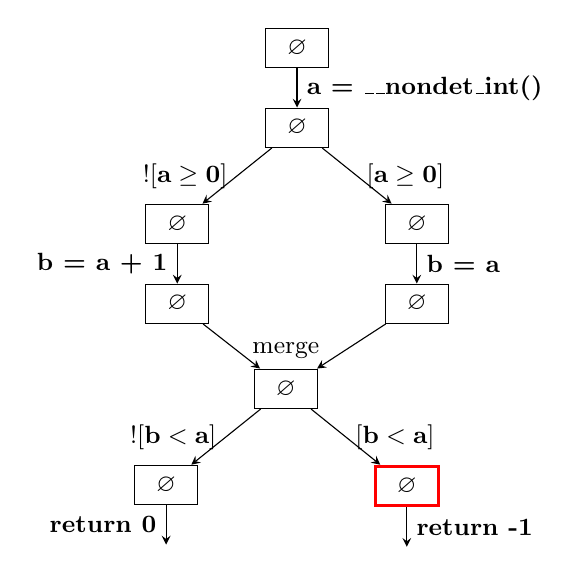
\begin{tikzpicture}[->,>=stealth, mynode/.style={rectangle, draw, minimum height=0.5cm, minimum width=0.8cm}, every node/.style={font=\small}]

  \node[mynode] (0) {$\varnothing$};
  \node[mynode] (1) [below = 0.5cm of 0]{$\varnothing$};
  \node[mynode] (2) [below left = 1cm of 1]{$\varnothing$};
  \node[mynode] (4) [below right = 1cm of 1]{$\varnothing$};
  \node[mynode] (3) [below = 0.5cm of 2]{$\varnothing$};
  \node[mynode] (5) [below = 0.5cm of 4]{$\varnothing$};
  \node[mynode] (6) [below right = 0.8cm of 3, label=north:merge]{$\varnothing$};
  \node[mynode] (7) [below left = 1cm of 6]{$\varnothing$};
  \node[mynode] (8) [below right = 1cm of 6, draw=red, very thick]{$\varnothing$};
  \coordinate[below = 0.5cm of 7] (e7);
  \coordinate[below = 0.5cm of 8] (e8);

  \path
    (0) edge node [right] {\textbf{a = \_\_nondet\_int()}} (1)
    (1) edge node [left, pos=0.5] {$\mathbf{![a \geq 0]}$} (2)
    (1) edge node [right, pos=0.5] {$\mathbf{[a \geq 0]}$} (4)
    (2) edge node [left] {\textbf{b = a + 1}} (3)
    (4) edge node [right] {\textbf{b = a}} (5)
    (3) edge (6)
    (5) edge (6)
    (6) edge node [left, pos=0.5] {$\mathbf{![b < a]}$} (7)
    (6) edge node [right, pos=0.5] {$\mathbf{[b < a]}$} (8)
    (7) edge node [left] {\textbf{return 0}} (e7)
    (8) edge node [right] {\textbf{return -1}} (e8)
  ;
\end{tikzpicture}
%\label{fig:ex1ValueGraph}
%\caption{Analysis of the program to the left by the \valueAnalysisCPA.}
\end{subfigure}
\caption{Simple program and its execution by the \valueAnalysisCPA.}
\label{fig:ex1}
\end{figure}

\begin{figure}[t]
\centering
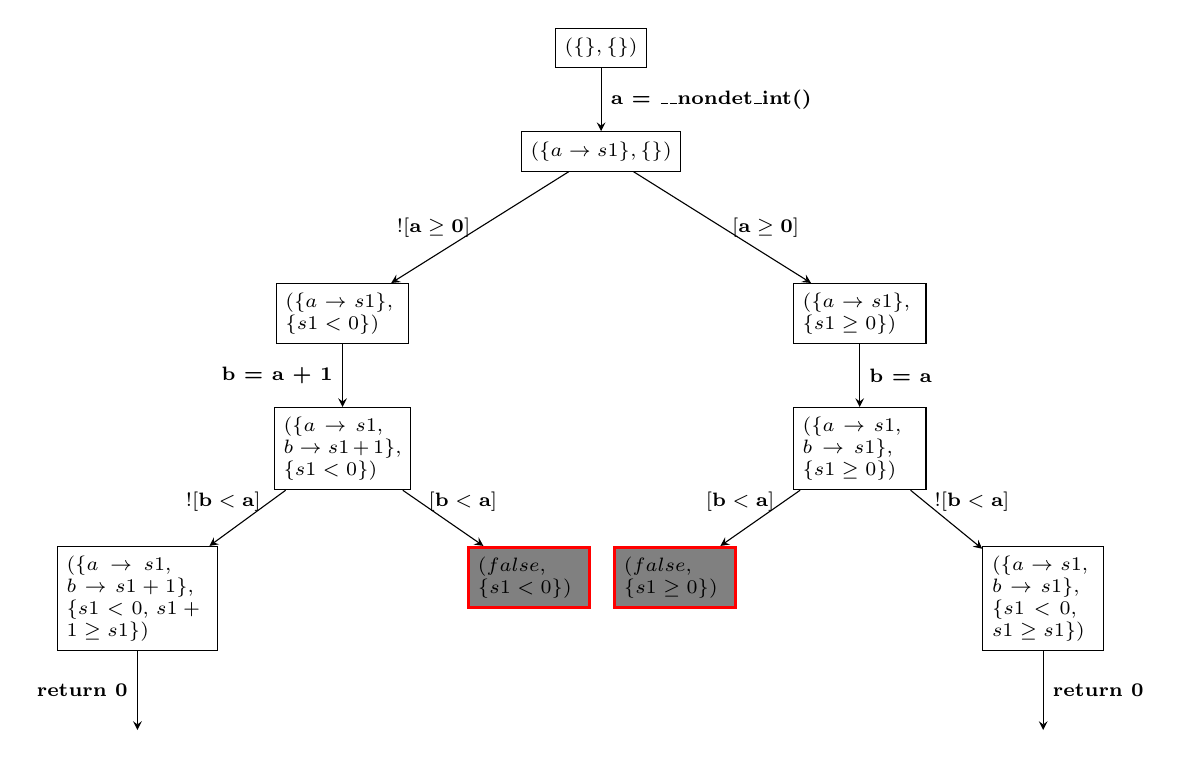
\begin{tikzpicture}[->,>=stealth, mynode/.style={rectangle, draw, minimum height=0.5cm, minimum width=0.8cm}, every node/.style={font=\scriptsize}]

  \node[mynode] (0) {$(\{\}, \{\})$};
  \node[mynode] (1) [below = 0.8cm of 0] {$(\{a \rightarrow s1\}, \{\})$};
  \node[mynode] (2) [below left = 2cm of 1, text width=1.45cm] {$(\{a \rightarrow s1\}$, $\{s1 < 0\})$};
  \node[mynode] (4) [below right = 2cm of 1, text width=1.45cm] {$(\{a \rightarrow s1\}$, $\{s1 \geq 0\})$};
  \node[mynode] (3) [below = 0.8cm of 2, text width=1.5cm] {$(\{a \rightarrow s1$, $b \rightarrow s1+1\}$, $\{s1 < 0\})$};
  \node[mynode] (5) [below = 0.8cm of 4, text width=1.45cm] {$(\{a \rightarrow s1$, $b \rightarrow s1 \}$, $\{s1 \geq 0\})$};
%  \node[mynode] (6) [below = 0.8cm of 3, text width=1.45cm] {$(\{a \rightarrow s1$, $b \rightarrow s1+1\}$, $\{s1 < 0\})$};
 % \node[mynode] (6n) [below = 0.8cm of 5, text width=1.45cm] {$(\{a \rightarrow s1$, $b \rightarrow s1 \}$, $\{s1 \geq 0\})$};
  \node[mynode] (7) [below left = 1cm of 3, text width=1.8cm] {$(\{a \rightarrow s1$, $b \rightarrow s1+1\}$, $\{s1 < 0$, $s1+1 \geq s1\})$};
  \node[mynode] (8) [below right = 1cm of 3, draw=red, fill=gray, very thick, text width=1.3cm]{$(false$, $\{s1 < 0\})$};
  \node[mynode] (8n) [below left = 1cm of 5, draw=red, fill=gray, very thick, text width=1.3cm]{$(false$, $\{s1 \geq 0\})$};
  \node[mynode] (7n) [below right = 1cm of 5, text width=1.3cm] {$(\{a \rightarrow s1$, $b \rightarrow s1\}$, $\{s1 < 0$, $s1 \geq s1\})$};
  \coordinate[below = 1cm of 7] (e7);
  \coordinate[below = 1cm of 7n] (e7n);

  \path
    (0) edge node [right] {\textbf{a = \_\_nondet\_int()}} (1)
    (1) edge node [left, pos=0.5] {$\mathbf{![a \geq 0]}$} (2)
    (1) edge node [right, pos=0.5] {$\mathbf{[a \geq 0]}$} (4)
    (2) edge node [left] {\textbf{b = a + 1}} (3)
    (4) edge node [right] {\textbf{b = a}} (5)
%    (3) edge (6)
%    (5) edge (6n)
    (3) edge node [left, pos=0.2] {$\mathbf{![b < a]}$} (7)
    (3) edge node [right, pos=0.2] {$\mathbf{[b < a]}$} (8)
    (5) edge node [left, pos=0.2] {$\mathbf{[b < a]}$} (8n)
    (5) edge node [right, pos=0.2] {$\mathbf{![b < a]}$} (7n)
    (7) edge node [left] {\textbf{return 0}} (e7)
    (7n) edge node [right] {\textbf{return 0}} (e7n)
  ;
\end{tikzpicture}
\caption{Analysis of the program in Listing \ref{lst:exProg} by the \symbolicExecutionCPA.}
\label{fig:ex1SymExGraph}
\end{figure}

%\subsubsection{Basic Value Analysis can't deal with non-deterministic values (+ Example)}
Figure \ref{fig:ex1} displays an example program that uses non-deterministic values and its analysis using the classic \valueAnalysisCPA.
Since the CPA does not store any information about non-deterministic assignments, no information about the relation between \textbf{a}\ and \textbf{b}\ exists and the property violation is reachable according to the analysis. This produces a \emph{false alarm}.
In constrast to this, the \symbolicExecutionCPA\ is able to handle the non-deterministic assignment to \textbf{a}\ a and its later usage. It returns that the program is safe, correctly.
Figure \ref{fig:ex1SymExGraph} shows this analysis. 

\SymbolicExecutionCPA's ability to track non-deterministic values is able to reduce the number of false alarms to a great extent, as we already showed in \cite{Lemberger2015}.
%\subsubsection{But symbolic value analysis pretty slow, as previous evaluation has shown (illustrate path explosion, sat checks)}
Runtime wise, it performs poorly, though, when compared to the \valueAnalysisCPA.
Since it considers all variable assignments, both deterministic and non-deterministic, and all occurring assumptions, its state space is exponential to the amount of occuring assumptions.
If a infinite loop occurs, the state space is infinite, too.
This problem is called \emph{path explosion}.\cite{Anand2008}
Obviously, an exponential amount of states does not scale to large programs.
In addition, the cost for SAT checks, which are performed at every assumption, are exponential to the amount of non-deterministic values occuring in all encountered assumptions on the currently considered program path.
Evaluation in \cite{Lemberger2015} showed that the \symbolicExecutionCPA\ spends up to 95\% of its runtime for SAT checks.

%\subsubsection{Goal: Try to speed up}
In this work we design, implement and evaluate different approaches to increasing the performance of the \symbolicExecutionCPA.
Our main contribution is, along with variations to the existing merge and less-or-equal operators of the CPA,
the application of CEGAR \cite{Clarke2003} to the composition of the two strongly intertwined CPAs \valueAnalysisCPA\ and \constraintsCPA\ with precision refinement for both CPAs
with two different precision types.

This work is divided into four parts: Theoretical background and contributions, their implementation, their evaluation, and future work and a conclusion.
First we will describe the concepts that are the basis for our work, such as Configurable Software Verification, used CPAs and CEGAR.
Next, we will illustrate the theory behind our own contribution,
before explaining details about the existing and newly added implementation and deviations from theory.
We will evaluate all presented concepts and compare them to the performance of the \valueAnalysisCPA, \predicateCPA, and \symbolicExecutionCPA\ of our old work.
Last, we will give a short outlook to possible future work in this field and close with a conclusion.
%%%%%%%%%%%%%%%%%%%%%%%%%%%%%%%
\section{Introduction}
%\subsubsection{Why Software Verification is important/needed}
Software systems are prone to error due to multiple factors: The developers skills, humans' limited understanding of software principles, communication problems in development, missing or sparse documentation and unforeseen interdependencies between software components are just some of them.

Because of this testing has been an integral part of software development for quite some time, often claiming about 50\% of development effort and more than 50\% of the budget.
\emph{Software testing} describes the execution of a program with the intention of finding errors.
The tester, either a person or another program, uses different inputs and checks that the proper output is produced.
The nature of this approach determines that only a finite amount of inputs is possible in finite time.
As a result, it is impossible to ensure the errorless execution of a program with arbitrary input.
Additionally, human testing is a technique only shortly touched in most software engineering educations, resembling art more than science.\cite{Myers2011}

Along with these points, the rise of ubiquitious computing and reactive systems complicates the process of reliable verification by testing even more.
Always running systems that gather, evaluate and adapt their behaviour to information of their environment pose an immense amount of possible inputs and interactions due to these.
This makes it almost impossible to predict the behaviour of such systems through testing.

An alternative to testing is formal verification, which tries to produce formal statements that are true for all possible behaviours of a system, using mathematical methods.
These statements are then used for proving that a specific specification is met.
One area of formal verification is \emph{automated software verification}. It tries to reach the above goal by only using software that works without the help or feedback of humans.
\CpaChecker\ \cite{Beyer2011} is such a program that yielded excellent performance in the last iterations of  the \href{http://sv-comp.sosy-lab.org}{Competition on Software Verification} (SV-COMP) \cite{SV-COMP2013} \cite{SV-COMP2014} \cite{SV-COMP2015}.
\CpaChecker\ is a framework for \emph{Configurable Software Verification} \cite{Beyer2007} utilizing different \emph{configurable program analyses} (CPAs) to locate possible property violations of a specification in a program.
Three such CPAs are the \valueAnalysisCPA, which uses concrete variable assignments, the \predicateCPA, which creates predicates for describing properties of program paths,
and the \symbolicExecutionCPA, which uses an extension of the \valueAnalysisCPA\ tracking non-deterministic values as symbolic ones in combination with the \constraintsCPA, which tracks constraints to symbolic values on program paths.
While the \valueAnalysisCPA\ has high efficiency due to her simplicity, it can't handle complex program characteristics like pointers or non-deterministic values.
The \predicateCPA, in constrast, is very expressive, but has low efficiency since SAT checks are necessary for computing the feasibility of a program path.
The \symbolicExecutionCPA\ poses something in between those two, not being able to handle some complex program characteristics as it is partly based on the \valueAnalysisCPA, but being able to handle non-deterministic values.
On the other hand, it uses SAT checks, too, though less often and over smaller formulas.

\begin{figure}[t]
\lstset{numbers=left}
\begin{subfigure}[b]{.45\textwidth}
\lstinputlisting[language=C]{exampleProgram.c}
%\caption{A simple non-deterministic program.}
%\label{lst:exProg}
\end{subfigure}%
\hfill
\begin{subfigure}[b]{.45\textwidth}
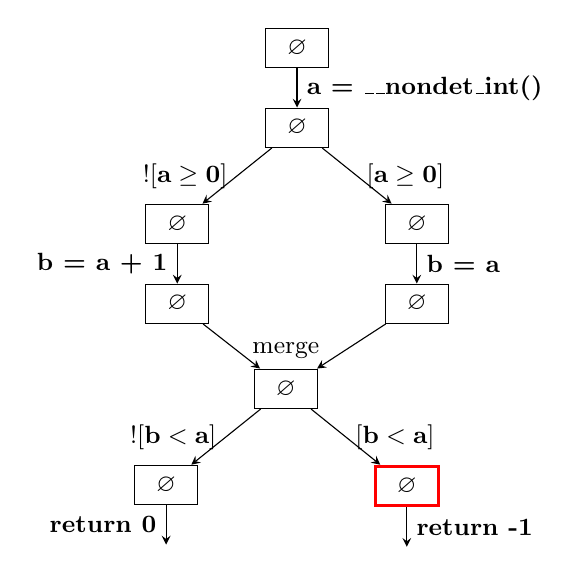
\begin{tikzpicture}[->,>=stealth, mynode/.style={rectangle, draw, minimum height=0.5cm, minimum width=0.8cm}, every node/.style={font=\small}]

  \node[mynode] (0) {$\varnothing$};
  \node[mynode] (1) [below = 0.5cm of 0]{$\varnothing$};
  \node[mynode] (2) [below left = 1cm of 1]{$\varnothing$};
  \node[mynode] (4) [below right = 1cm of 1]{$\varnothing$};
  \node[mynode] (3) [below = 0.5cm of 2]{$\varnothing$};
  \node[mynode] (5) [below = 0.5cm of 4]{$\varnothing$};
  \node[mynode] (6) [below right = 0.8cm of 3, label=north:merge]{$\varnothing$};
  \node[mynode] (7) [below left = 1cm of 6]{$\varnothing$};
  \node[mynode] (8) [below right = 1cm of 6, draw=red, very thick]{$\varnothing$};
  \coordinate[below = 0.5cm of 7] (e7);
  \coordinate[below = 0.5cm of 8] (e8);

  \path
    (0) edge node [right] {\textbf{a = \_\_nondet\_int()}} (1)
    (1) edge node [left, pos=0.5] {$\mathbf{![a \geq 0]}$} (2)
    (1) edge node [right, pos=0.5] {$\mathbf{[a \geq 0]}$} (4)
    (2) edge node [left] {\textbf{b = a + 1}} (3)
    (4) edge node [right] {\textbf{b = a}} (5)
    (3) edge (6)
    (5) edge (6)
    (6) edge node [left, pos=0.5] {$\mathbf{![b < a]}$} (7)
    (6) edge node [right, pos=0.5] {$\mathbf{[b < a]}$} (8)
    (7) edge node [left] {\textbf{return 0}} (e7)
    (8) edge node [right] {\textbf{return -1}} (e8)
  ;
\end{tikzpicture}
%\label{fig:ex1ValueGraph}
%\caption{Analysis of the program to the left by the \valueAnalysisCPA.}
\end{subfigure}
\caption{Simple program and its execution by the \valueAnalysisCPA.}
\label{fig:ex1}
\end{figure}

\begin{figure}[t]
\centering
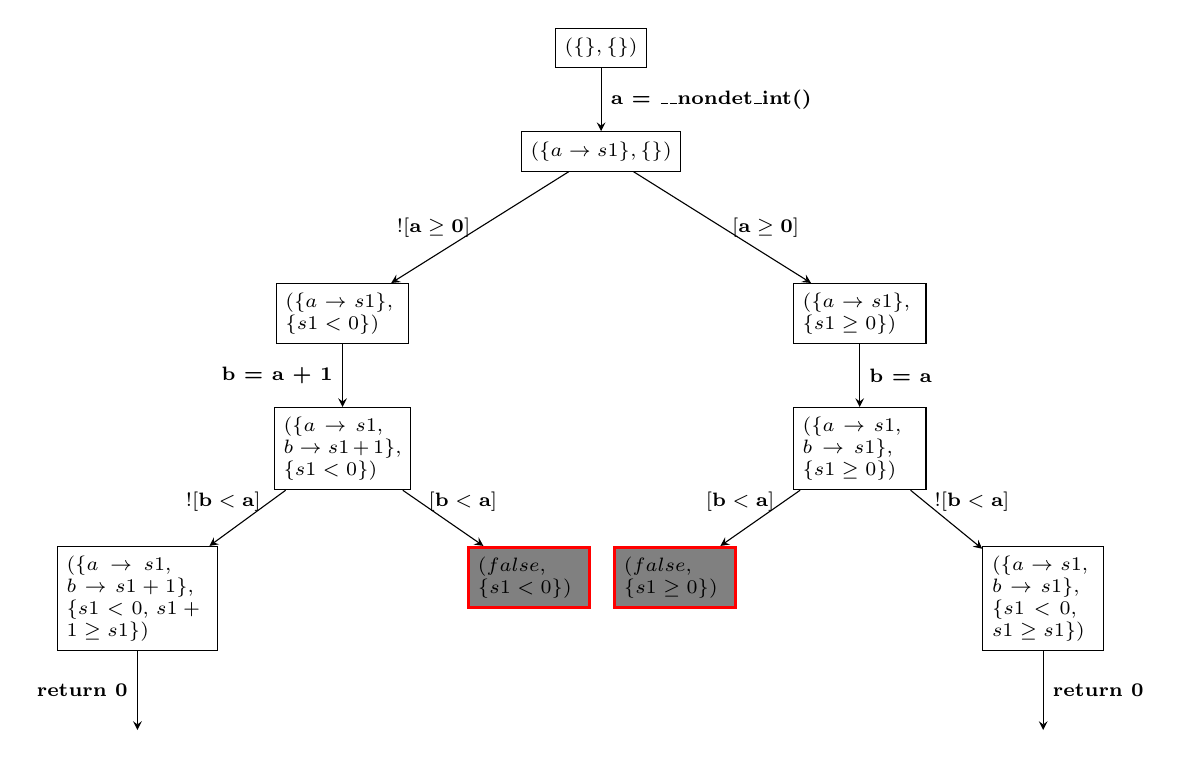
\begin{tikzpicture}[->,>=stealth, mynode/.style={rectangle, draw, minimum height=0.5cm, minimum width=0.8cm}, every node/.style={font=\scriptsize}]

  \node[mynode] (0) {$(\{\}, \{\})$};
  \node[mynode] (1) [below = 0.8cm of 0] {$(\{a \rightarrow s1\}, \{\})$};
  \node[mynode] (2) [below left = 2cm of 1, text width=1.45cm] {$(\{a \rightarrow s1\}$, $\{s1 < 0\})$};
  \node[mynode] (4) [below right = 2cm of 1, text width=1.45cm] {$(\{a \rightarrow s1\}$, $\{s1 \geq 0\})$};
  \node[mynode] (3) [below = 0.8cm of 2, text width=1.5cm] {$(\{a \rightarrow s1$, $b \rightarrow s1+1\}$, $\{s1 < 0\})$};
  \node[mynode] (5) [below = 0.8cm of 4, text width=1.45cm] {$(\{a \rightarrow s1$, $b \rightarrow s1 \}$, $\{s1 \geq 0\})$};
%  \node[mynode] (6) [below = 0.8cm of 3, text width=1.45cm] {$(\{a \rightarrow s1$, $b \rightarrow s1+1\}$, $\{s1 < 0\})$};
 % \node[mynode] (6n) [below = 0.8cm of 5, text width=1.45cm] {$(\{a \rightarrow s1$, $b \rightarrow s1 \}$, $\{s1 \geq 0\})$};
  \node[mynode] (7) [below left = 1cm of 3, text width=1.8cm] {$(\{a \rightarrow s1$, $b \rightarrow s1+1\}$, $\{s1 < 0$, $s1+1 \geq s1\})$};
  \node[mynode] (8) [below right = 1cm of 3, draw=red, fill=gray, very thick, text width=1.3cm]{$(false$, $\{s1 < 0\})$};
  \node[mynode] (8n) [below left = 1cm of 5, draw=red, fill=gray, very thick, text width=1.3cm]{$(false$, $\{s1 \geq 0\})$};
  \node[mynode] (7n) [below right = 1cm of 5, text width=1.3cm] {$(\{a \rightarrow s1$, $b \rightarrow s1\}$, $\{s1 < 0$, $s1 \geq s1\})$};
  \coordinate[below = 1cm of 7] (e7);
  \coordinate[below = 1cm of 7n] (e7n);

  \path
    (0) edge node [right] {\textbf{a = \_\_nondet\_int()}} (1)
    (1) edge node [left, pos=0.5] {$\mathbf{![a \geq 0]}$} (2)
    (1) edge node [right, pos=0.5] {$\mathbf{[a \geq 0]}$} (4)
    (2) edge node [left] {\textbf{b = a + 1}} (3)
    (4) edge node [right] {\textbf{b = a}} (5)
%    (3) edge (6)
%    (5) edge (6n)
    (3) edge node [left, pos=0.2] {$\mathbf{![b < a]}$} (7)
    (3) edge node [right, pos=0.2] {$\mathbf{[b < a]}$} (8)
    (5) edge node [left, pos=0.2] {$\mathbf{[b < a]}$} (8n)
    (5) edge node [right, pos=0.2] {$\mathbf{![b < a]}$} (7n)
    (7) edge node [left] {\textbf{return 0}} (e7)
    (7n) edge node [right] {\textbf{return 0}} (e7n)
  ;
\end{tikzpicture}
\caption{Analysis of the program in Listing \ref{lst:exProg} by the \symbolicExecutionCPA.}
\label{fig:ex1SymExGraph}
\end{figure}

%\subsubsection{Basic Value Analysis can't deal with non-deterministic values (+ Example)}
Figure \ref{fig:ex1} displays an example program that uses non-deterministic values and its analysis using the classic \valueAnalysisCPA.
Since the CPA does not store any information about non-deterministic assignments, no information about the relation between \textbf{a}\ and \textbf{b}\ exists and the property violation is reachable according to the analysis. This produces a \emph{false alarm}.
In constrast to this, the \symbolicExecutionCPA\ is able to handle the non-deterministic assignment to \textbf{a}\ a and its later usage. It returns that the program is safe, correctly.
Figure \ref{fig:ex1SymExGraph} shows this analysis. 

\SymbolicExecutionCPA's ability to track non-deterministic values is able to reduce the number of false alarms to a great extent, as we already showed in \cite{Lemberger2015}.
%\subsubsection{But symbolic value analysis pretty slow, as previous evaluation has shown (illustrate path explosion, sat checks)}
Runtime wise, it performs poorly, though, when compared to the \valueAnalysisCPA.
Since it considers all variable assignments, both deterministic and non-deterministic, and all occurring assumptions, its state space is exponential to the amount of occuring assumptions.
If a infinite loop occurs, the state space is infinite, too.
This problem is called \emph{path explosion}.\cite{Anand2008}
Obviously, an exponential amount of states does not scale to large programs.
In addition, the cost for SAT checks, which are performed at every assumption, are exponential to the amount of non-deterministic values occuring in all encountered assumptions on the currently considered program path.
Evaluation in \cite{Lemberger2015} showed that the \symbolicExecutionCPA\ spends up to 95\% of its runtime for SAT checks.

%\subsubsection{Goal: Try to speed up}
In this work we design, implement and evaluate different approaches to increasing the performance of the \symbolicExecutionCPA.
Our main contribution is, along with variations to the existing merge and less-or-equal operators of the CPA,
the application of CEGAR \cite{Clarke2003} to the composition of the two strongly intertwined CPAs \valueAnalysisCPA\ and \constraintsCPA\ with precision refinement for both CPAs
with two different precision types.

This work is divided into four parts: Theoretical background and contributions, their implementation, their evaluation, and future work and a conclusion.
First we will describe the concepts that are the basis for our work, such as Configurable Software Verification, used CPAs and CEGAR.
Next, we will illustrate the theory behind our own contribution,
before explaining details about the existing and newly added implementation and deviations from theory.
We will evaluate all presented concepts and compare them to the performance of the \valueAnalysisCPA, \predicateCPA, and \symbolicExecutionCPA\ of our old work.
Last, we will give a short outlook to possible future work in this field and close with a conclusion.
%%%%%%%%%%%%%%%%%%%%%%%%
%\section{Introduction}
%\subsubsection{Why Software Verification is important/needed}
Software systems are prone to error due to multiple factors: The developers skills, humans' limited understanding of software principles, communication problems in development, missing or sparse documentation and unforeseen interdependencies between software components are just some of them.

Because of this testing has been an integral part of software development for quite some time, often claiming about 50\% of development effort and more than 50\% of the budget.
\emph{Software testing} describes the execution of a program with the intention of finding errors.
The tester, either a person or another program, uses different inputs and checks that the proper output is produced.
The nature of this approach determines that only a finite amount of inputs is possible in finite time.
As a result, it is impossible to ensure the errorless execution of a program with arbitrary input.
Additionally, human testing is a technique only shortly touched in most software engineering educations, resembling art more than science.\cite{Myers2011}

Along with these points, the rise of ubiquitious computing and reactive systems complicates the process of reliable verification by testing even more.
Always running systems that gather, evaluate and adapt their behaviour to information of their environment pose an immense amount of possible inputs and interactions due to these.
This makes it almost impossible to predict the behaviour of such systems through testing.

An alternative to testing is formal verification, which tries to produce formal statements that are true for all possible behaviours of a system, using mathematical methods.
These statements are then used for proving that a specific specification is met.
One area of formal verification is \emph{automated software verification}. It tries to reach the above goal by only using software that works without the help or feedback of humans.
\CpaChecker\ \cite{Beyer2011} is such a program that yielded excellent performance in the last iterations of  the \href{http://sv-comp.sosy-lab.org}{Competition on Software Verification} (SV-COMP) \cite{SV-COMP2013} \cite{SV-COMP2014} \cite{SV-COMP2015}.
\CpaChecker\ is a framework for \emph{Configurable Software Verification} \cite{Beyer2007} utilizing different \emph{configurable program analyses} (CPAs) to locate possible property violations of a specification in a program.
Three such CPAs are the \valueAnalysisCPA, which uses concrete variable assignments, the \predicateCPA, which creates predicates for describing properties of program paths,
and the \symbolicExecutionCPA, which uses an extension of the \valueAnalysisCPA\ tracking non-deterministic values as symbolic ones in combination with the \constraintsCPA, which tracks constraints to symbolic values on program paths.
While the \valueAnalysisCPA\ has high efficiency due to her simplicity, it can't handle complex program characteristics like pointers or non-deterministic values.
The \predicateCPA, in constrast, is very expressive, but has low efficiency since SAT checks are necessary for computing the feasibility of a program path.
The \symbolicExecutionCPA\ poses something in between those two, not being able to handle some complex program characteristics as it is partly based on the \valueAnalysisCPA, but being able to handle non-deterministic values.
On the other hand, it uses SAT checks, too, though less often and over smaller formulas.

\begin{figure}[t]
\lstset{numbers=left}
\begin{subfigure}[b]{.45\textwidth}
\lstinputlisting[language=C]{exampleProgram.c}
%\caption{A simple non-deterministic program.}
%\label{lst:exProg}
\end{subfigure}%
\hfill
\begin{subfigure}[b]{.45\textwidth}
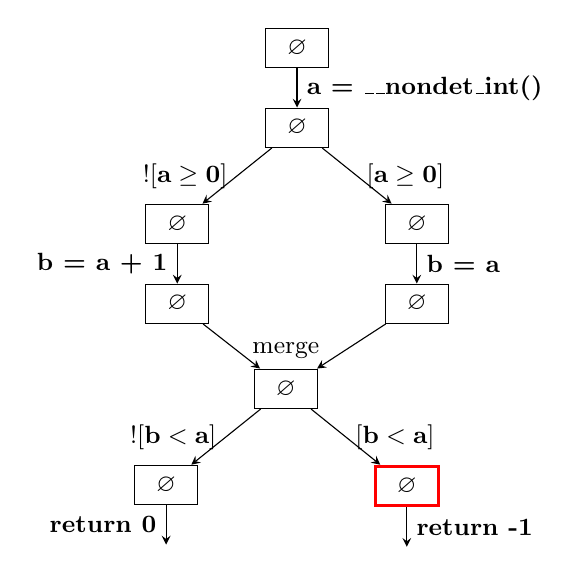
\begin{tikzpicture}[->,>=stealth, mynode/.style={rectangle, draw, minimum height=0.5cm, minimum width=0.8cm}, every node/.style={font=\small}]

  \node[mynode] (0) {$\varnothing$};
  \node[mynode] (1) [below = 0.5cm of 0]{$\varnothing$};
  \node[mynode] (2) [below left = 1cm of 1]{$\varnothing$};
  \node[mynode] (4) [below right = 1cm of 1]{$\varnothing$};
  \node[mynode] (3) [below = 0.5cm of 2]{$\varnothing$};
  \node[mynode] (5) [below = 0.5cm of 4]{$\varnothing$};
  \node[mynode] (6) [below right = 0.8cm of 3, label=north:merge]{$\varnothing$};
  \node[mynode] (7) [below left = 1cm of 6]{$\varnothing$};
  \node[mynode] (8) [below right = 1cm of 6, draw=red, very thick]{$\varnothing$};
  \coordinate[below = 0.5cm of 7] (e7);
  \coordinate[below = 0.5cm of 8] (e8);

  \path
    (0) edge node [right] {\textbf{a = \_\_nondet\_int()}} (1)
    (1) edge node [left, pos=0.5] {$\mathbf{![a \geq 0]}$} (2)
    (1) edge node [right, pos=0.5] {$\mathbf{[a \geq 0]}$} (4)
    (2) edge node [left] {\textbf{b = a + 1}} (3)
    (4) edge node [right] {\textbf{b = a}} (5)
    (3) edge (6)
    (5) edge (6)
    (6) edge node [left, pos=0.5] {$\mathbf{![b < a]}$} (7)
    (6) edge node [right, pos=0.5] {$\mathbf{[b < a]}$} (8)
    (7) edge node [left] {\textbf{return 0}} (e7)
    (8) edge node [right] {\textbf{return -1}} (e8)
  ;
\end{tikzpicture}
%\label{fig:ex1ValueGraph}
%\caption{Analysis of the program to the left by the \valueAnalysisCPA.}
\end{subfigure}
\caption{Simple program and its execution by the \valueAnalysisCPA.}
\label{fig:ex1}
\end{figure}

\begin{figure}[t]
\centering
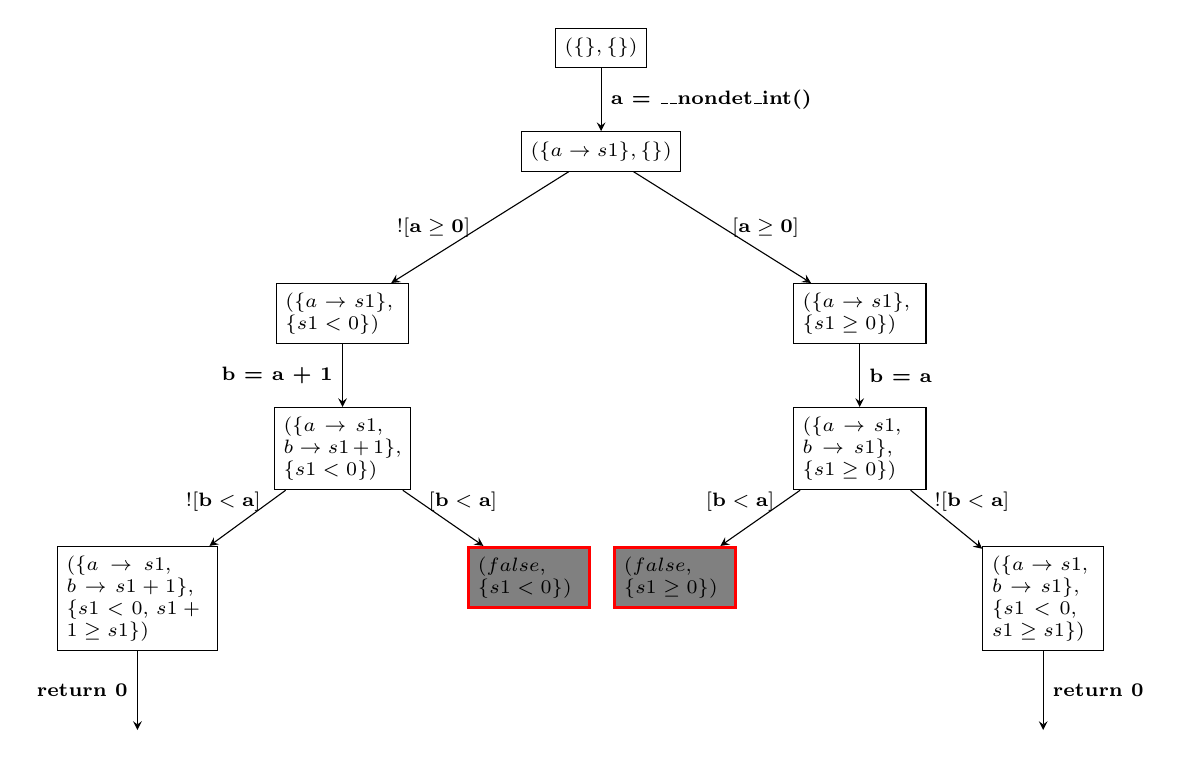
\begin{tikzpicture}[->,>=stealth, mynode/.style={rectangle, draw, minimum height=0.5cm, minimum width=0.8cm}, every node/.style={font=\scriptsize}]

  \node[mynode] (0) {$(\{\}, \{\})$};
  \node[mynode] (1) [below = 0.8cm of 0] {$(\{a \rightarrow s1\}, \{\})$};
  \node[mynode] (2) [below left = 2cm of 1, text width=1.45cm] {$(\{a \rightarrow s1\}$, $\{s1 < 0\})$};
  \node[mynode] (4) [below right = 2cm of 1, text width=1.45cm] {$(\{a \rightarrow s1\}$, $\{s1 \geq 0\})$};
  \node[mynode] (3) [below = 0.8cm of 2, text width=1.5cm] {$(\{a \rightarrow s1$, $b \rightarrow s1+1\}$, $\{s1 < 0\})$};
  \node[mynode] (5) [below = 0.8cm of 4, text width=1.45cm] {$(\{a \rightarrow s1$, $b \rightarrow s1 \}$, $\{s1 \geq 0\})$};
%  \node[mynode] (6) [below = 0.8cm of 3, text width=1.45cm] {$(\{a \rightarrow s1$, $b \rightarrow s1+1\}$, $\{s1 < 0\})$};
 % \node[mynode] (6n) [below = 0.8cm of 5, text width=1.45cm] {$(\{a \rightarrow s1$, $b \rightarrow s1 \}$, $\{s1 \geq 0\})$};
  \node[mynode] (7) [below left = 1cm of 3, text width=1.8cm] {$(\{a \rightarrow s1$, $b \rightarrow s1+1\}$, $\{s1 < 0$, $s1+1 \geq s1\})$};
  \node[mynode] (8) [below right = 1cm of 3, draw=red, fill=gray, very thick, text width=1.3cm]{$(false$, $\{s1 < 0\})$};
  \node[mynode] (8n) [below left = 1cm of 5, draw=red, fill=gray, very thick, text width=1.3cm]{$(false$, $\{s1 \geq 0\})$};
  \node[mynode] (7n) [below right = 1cm of 5, text width=1.3cm] {$(\{a \rightarrow s1$, $b \rightarrow s1\}$, $\{s1 < 0$, $s1 \geq s1\})$};
  \coordinate[below = 1cm of 7] (e7);
  \coordinate[below = 1cm of 7n] (e7n);

  \path
    (0) edge node [right] {\textbf{a = \_\_nondet\_int()}} (1)
    (1) edge node [left, pos=0.5] {$\mathbf{![a \geq 0]}$} (2)
    (1) edge node [right, pos=0.5] {$\mathbf{[a \geq 0]}$} (4)
    (2) edge node [left] {\textbf{b = a + 1}} (3)
    (4) edge node [right] {\textbf{b = a}} (5)
%    (3) edge (6)
%    (5) edge (6n)
    (3) edge node [left, pos=0.2] {$\mathbf{![b < a]}$} (7)
    (3) edge node [right, pos=0.2] {$\mathbf{[b < a]}$} (8)
    (5) edge node [left, pos=0.2] {$\mathbf{[b < a]}$} (8n)
    (5) edge node [right, pos=0.2] {$\mathbf{![b < a]}$} (7n)
    (7) edge node [left] {\textbf{return 0}} (e7)
    (7n) edge node [right] {\textbf{return 0}} (e7n)
  ;
\end{tikzpicture}
\caption{Analysis of the program in Listing \ref{lst:exProg} by the \symbolicExecutionCPA.}
\label{fig:ex1SymExGraph}
\end{figure}

%\subsubsection{Basic Value Analysis can't deal with non-deterministic values (+ Example)}
Figure \ref{fig:ex1} displays an example program that uses non-deterministic values and its analysis using the classic \valueAnalysisCPA.
Since the CPA does not store any information about non-deterministic assignments, no information about the relation between \textbf{a}\ and \textbf{b}\ exists and the property violation is reachable according to the analysis. This produces a \emph{false alarm}.
In constrast to this, the \symbolicExecutionCPA\ is able to handle the non-deterministic assignment to \textbf{a}\ a and its later usage. It returns that the program is safe, correctly.
Figure \ref{fig:ex1SymExGraph} shows this analysis. 

\SymbolicExecutionCPA's ability to track non-deterministic values is able to reduce the number of false alarms to a great extent, as we already showed in \cite{Lemberger2015}.
%\subsubsection{But symbolic value analysis pretty slow, as previous evaluation has shown (illustrate path explosion, sat checks)}
Runtime wise, it performs poorly, though, when compared to the \valueAnalysisCPA.
Since it considers all variable assignments, both deterministic and non-deterministic, and all occurring assumptions, its state space is exponential to the amount of occuring assumptions.
If a infinite loop occurs, the state space is infinite, too.
This problem is called \emph{path explosion}.\cite{Anand2008}
Obviously, an exponential amount of states does not scale to large programs.
In addition, the cost for SAT checks, which are performed at every assumption, are exponential to the amount of non-deterministic values occuring in all encountered assumptions on the currently considered program path.
Evaluation in \cite{Lemberger2015} showed that the \symbolicExecutionCPA\ spends up to 95\% of its runtime for SAT checks.

%\subsubsection{Goal: Try to speed up}
In this work we design, implement and evaluate different approaches to increasing the performance of the \symbolicExecutionCPA.
Our main contribution is, along with variations to the existing merge and less-or-equal operators of the CPA,
the application of CEGAR \cite{Clarke2003} to the composition of the two strongly intertwined CPAs \valueAnalysisCPA\ and \constraintsCPA\ with precision refinement for both CPAs
with two different precision types.

This work is divided into four parts: Theoretical background and contributions, their implementation, their evaluation, and future work and a conclusion.
First we will describe the concepts that are the basis for our work, such as Configurable Software Verification, used CPAs and CEGAR.
Next, we will illustrate the theory behind our own contribution,
before explaining details about the existing and newly added implementation and deviations from theory.
We will evaluate all presented concepts and compare them to the performance of the \valueAnalysisCPA, \predicateCPA, and \symbolicExecutionCPA\ of our old work.
Last, we will give a short outlook to possible future work in this field and close with a conclusion.
%%%%%%%%%%%%%%%%%%%%%%%%%%%%%%%%
\section{Introduction}
%\subsubsection{Why Software Verification is important/needed}
Software systems are prone to error due to multiple factors: The developers skills, humans' limited understanding of software principles, communication problems in development, missing or sparse documentation and unforeseen interdependencies between software components are just some of them.

Because of this testing has been an integral part of software development for quite some time, often claiming about 50\% of development effort and more than 50\% of the budget.
\emph{Software testing} describes the execution of a program with the intention of finding errors.
The tester, either a person or another program, uses different inputs and checks that the proper output is produced.
The nature of this approach determines that only a finite amount of inputs is possible in finite time.
As a result, it is impossible to ensure the errorless execution of a program with arbitrary input.
Additionally, human testing is a technique only shortly touched in most software engineering educations, resembling art more than science.\cite{Myers2011}

Along with these points, the rise of ubiquitious computing and reactive systems complicates the process of reliable verification by testing even more.
Always running systems that gather, evaluate and adapt their behaviour to information of their environment pose an immense amount of possible inputs and interactions due to these.
This makes it almost impossible to predict the behaviour of such systems through testing.

An alternative to testing is formal verification, which tries to produce formal statements that are true for all possible behaviours of a system, using mathematical methods.
These statements are then used for proving that a specific specification is met.
One area of formal verification is \emph{automated software verification}. It tries to reach the above goal by only using software that works without the help or feedback of humans.
\CpaChecker\ \cite{Beyer2011} is such a program that yielded excellent performance in the last iterations of  the \href{http://sv-comp.sosy-lab.org}{Competition on Software Verification} (SV-COMP) \cite{SV-COMP2013} \cite{SV-COMP2014} \cite{SV-COMP2015}.
\CpaChecker\ is a framework for \emph{Configurable Software Verification} \cite{Beyer2007} utilizing different \emph{configurable program analyses} (CPAs) to locate possible property violations of a specification in a program.
Three such CPAs are the \valueAnalysisCPA, which uses concrete variable assignments, the \predicateCPA, which creates predicates for describing properties of program paths,
and the \symbolicExecutionCPA, which uses an extension of the \valueAnalysisCPA\ tracking non-deterministic values as symbolic ones in combination with the \constraintsCPA, which tracks constraints to symbolic values on program paths.
While the \valueAnalysisCPA\ has high efficiency due to her simplicity, it can't handle complex program characteristics like pointers or non-deterministic values.
The \predicateCPA, in constrast, is very expressive, but has low efficiency since SAT checks are necessary for computing the feasibility of a program path.
The \symbolicExecutionCPA\ poses something in between those two, not being able to handle some complex program characteristics as it is partly based on the \valueAnalysisCPA, but being able to handle non-deterministic values.
On the other hand, it uses SAT checks, too, though less often and over smaller formulas.

\begin{figure}[t]
\lstset{numbers=left}
\begin{subfigure}[b]{.45\textwidth}
\lstinputlisting[language=C]{exampleProgram.c}
%\caption{A simple non-deterministic program.}
%\label{lst:exProg}
\end{subfigure}%
\hfill
\begin{subfigure}[b]{.45\textwidth}
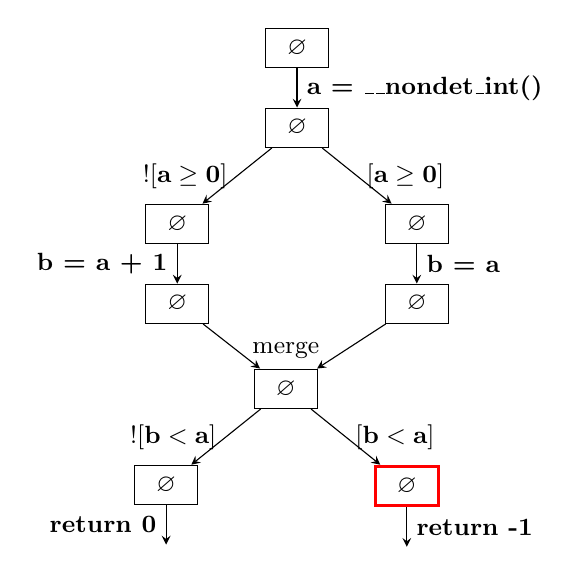
\begin{tikzpicture}[->,>=stealth, mynode/.style={rectangle, draw, minimum height=0.5cm, minimum width=0.8cm}, every node/.style={font=\small}]

  \node[mynode] (0) {$\varnothing$};
  \node[mynode] (1) [below = 0.5cm of 0]{$\varnothing$};
  \node[mynode] (2) [below left = 1cm of 1]{$\varnothing$};
  \node[mynode] (4) [below right = 1cm of 1]{$\varnothing$};
  \node[mynode] (3) [below = 0.5cm of 2]{$\varnothing$};
  \node[mynode] (5) [below = 0.5cm of 4]{$\varnothing$};
  \node[mynode] (6) [below right = 0.8cm of 3, label=north:merge]{$\varnothing$};
  \node[mynode] (7) [below left = 1cm of 6]{$\varnothing$};
  \node[mynode] (8) [below right = 1cm of 6, draw=red, very thick]{$\varnothing$};
  \coordinate[below = 0.5cm of 7] (e7);
  \coordinate[below = 0.5cm of 8] (e8);

  \path
    (0) edge node [right] {\textbf{a = \_\_nondet\_int()}} (1)
    (1) edge node [left, pos=0.5] {$\mathbf{![a \geq 0]}$} (2)
    (1) edge node [right, pos=0.5] {$\mathbf{[a \geq 0]}$} (4)
    (2) edge node [left] {\textbf{b = a + 1}} (3)
    (4) edge node [right] {\textbf{b = a}} (5)
    (3) edge (6)
    (5) edge (6)
    (6) edge node [left, pos=0.5] {$\mathbf{![b < a]}$} (7)
    (6) edge node [right, pos=0.5] {$\mathbf{[b < a]}$} (8)
    (7) edge node [left] {\textbf{return 0}} (e7)
    (8) edge node [right] {\textbf{return -1}} (e8)
  ;
\end{tikzpicture}
%\label{fig:ex1ValueGraph}
%\caption{Analysis of the program to the left by the \valueAnalysisCPA.}
\end{subfigure}
\caption{Simple program and its execution by the \valueAnalysisCPA.}
\label{fig:ex1}
\end{figure}

\begin{figure}[t]
\centering
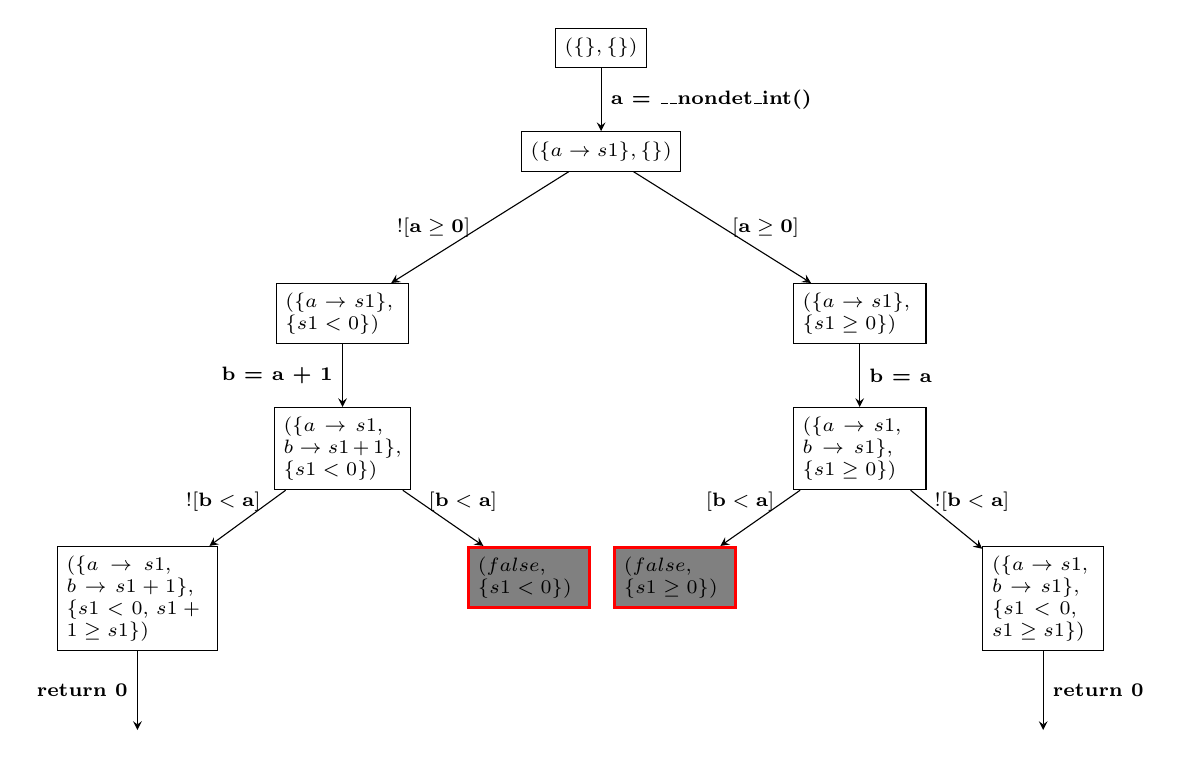
\begin{tikzpicture}[->,>=stealth, mynode/.style={rectangle, draw, minimum height=0.5cm, minimum width=0.8cm}, every node/.style={font=\scriptsize}]

  \node[mynode] (0) {$(\{\}, \{\})$};
  \node[mynode] (1) [below = 0.8cm of 0] {$(\{a \rightarrow s1\}, \{\})$};
  \node[mynode] (2) [below left = 2cm of 1, text width=1.45cm] {$(\{a \rightarrow s1\}$, $\{s1 < 0\})$};
  \node[mynode] (4) [below right = 2cm of 1, text width=1.45cm] {$(\{a \rightarrow s1\}$, $\{s1 \geq 0\})$};
  \node[mynode] (3) [below = 0.8cm of 2, text width=1.5cm] {$(\{a \rightarrow s1$, $b \rightarrow s1+1\}$, $\{s1 < 0\})$};
  \node[mynode] (5) [below = 0.8cm of 4, text width=1.45cm] {$(\{a \rightarrow s1$, $b \rightarrow s1 \}$, $\{s1 \geq 0\})$};
%  \node[mynode] (6) [below = 0.8cm of 3, text width=1.45cm] {$(\{a \rightarrow s1$, $b \rightarrow s1+1\}$, $\{s1 < 0\})$};
 % \node[mynode] (6n) [below = 0.8cm of 5, text width=1.45cm] {$(\{a \rightarrow s1$, $b \rightarrow s1 \}$, $\{s1 \geq 0\})$};
  \node[mynode] (7) [below left = 1cm of 3, text width=1.8cm] {$(\{a \rightarrow s1$, $b \rightarrow s1+1\}$, $\{s1 < 0$, $s1+1 \geq s1\})$};
  \node[mynode] (8) [below right = 1cm of 3, draw=red, fill=gray, very thick, text width=1.3cm]{$(false$, $\{s1 < 0\})$};
  \node[mynode] (8n) [below left = 1cm of 5, draw=red, fill=gray, very thick, text width=1.3cm]{$(false$, $\{s1 \geq 0\})$};
  \node[mynode] (7n) [below right = 1cm of 5, text width=1.3cm] {$(\{a \rightarrow s1$, $b \rightarrow s1\}$, $\{s1 < 0$, $s1 \geq s1\})$};
  \coordinate[below = 1cm of 7] (e7);
  \coordinate[below = 1cm of 7n] (e7n);

  \path
    (0) edge node [right] {\textbf{a = \_\_nondet\_int()}} (1)
    (1) edge node [left, pos=0.5] {$\mathbf{![a \geq 0]}$} (2)
    (1) edge node [right, pos=0.5] {$\mathbf{[a \geq 0]}$} (4)
    (2) edge node [left] {\textbf{b = a + 1}} (3)
    (4) edge node [right] {\textbf{b = a}} (5)
%    (3) edge (6)
%    (5) edge (6n)
    (3) edge node [left, pos=0.2] {$\mathbf{![b < a]}$} (7)
    (3) edge node [right, pos=0.2] {$\mathbf{[b < a]}$} (8)
    (5) edge node [left, pos=0.2] {$\mathbf{[b < a]}$} (8n)
    (5) edge node [right, pos=0.2] {$\mathbf{![b < a]}$} (7n)
    (7) edge node [left] {\textbf{return 0}} (e7)
    (7n) edge node [right] {\textbf{return 0}} (e7n)
  ;
\end{tikzpicture}
\caption{Analysis of the program in Listing \ref{lst:exProg} by the \symbolicExecutionCPA.}
\label{fig:ex1SymExGraph}
\end{figure}

%\subsubsection{Basic Value Analysis can't deal with non-deterministic values (+ Example)}
Figure \ref{fig:ex1} displays an example program that uses non-deterministic values and its analysis using the classic \valueAnalysisCPA.
Since the CPA does not store any information about non-deterministic assignments, no information about the relation between \textbf{a}\ and \textbf{b}\ exists and the property violation is reachable according to the analysis. This produces a \emph{false alarm}.
In constrast to this, the \symbolicExecutionCPA\ is able to handle the non-deterministic assignment to \textbf{a}\ a and its later usage. It returns that the program is safe, correctly.
Figure \ref{fig:ex1SymExGraph} shows this analysis. 

\SymbolicExecutionCPA's ability to track non-deterministic values is able to reduce the number of false alarms to a great extent, as we already showed in \cite{Lemberger2015}.
%\subsubsection{But symbolic value analysis pretty slow, as previous evaluation has shown (illustrate path explosion, sat checks)}
Runtime wise, it performs poorly, though, when compared to the \valueAnalysisCPA.
Since it considers all variable assignments, both deterministic and non-deterministic, and all occurring assumptions, its state space is exponential to the amount of occuring assumptions.
If a infinite loop occurs, the state space is infinite, too.
This problem is called \emph{path explosion}.\cite{Anand2008}
Obviously, an exponential amount of states does not scale to large programs.
In addition, the cost for SAT checks, which are performed at every assumption, are exponential to the amount of non-deterministic values occuring in all encountered assumptions on the currently considered program path.
Evaluation in \cite{Lemberger2015} showed that the \symbolicExecutionCPA\ spends up to 95\% of its runtime for SAT checks.

%\subsubsection{Goal: Try to speed up}
In this work we design, implement and evaluate different approaches to increasing the performance of the \symbolicExecutionCPA.
Our main contribution is, along with variations to the existing merge and less-or-equal operators of the CPA,
the application of CEGAR \cite{Clarke2003} to the composition of the two strongly intertwined CPAs \valueAnalysisCPA\ and \constraintsCPA\ with precision refinement for both CPAs
with two different precision types.

This work is divided into four parts: Theoretical background and contributions, their implementation, their evaluation, and future work and a conclusion.
First we will describe the concepts that are the basis for our work, such as Configurable Software Verification, used CPAs and CEGAR.
Next, we will illustrate the theory behind our own contribution,
before explaining details about the existing and newly added implementation and deviations from theory.
We will evaluate all presented concepts and compare them to the performance of the \valueAnalysisCPA, \predicateCPA, and \symbolicExecutionCPA\ of our old work.
Last, we will give a short outlook to possible future work in this field and close with a conclusion.
%%%%%%%%%%%%%%%%%%%%%%%%%%%%%%%%
\section{Introduction}
%\subsubsection{Why Software Verification is important/needed}
Software systems are prone to error due to multiple factors: The developers skills, humans' limited understanding of software principles, communication problems in development, missing or sparse documentation and unforeseen interdependencies between software components are just some of them.

Because of this testing has been an integral part of software development for quite some time, often claiming about 50\% of development effort and more than 50\% of the budget.
\emph{Software testing} describes the execution of a program with the intention of finding errors.
The tester, either a person or another program, uses different inputs and checks that the proper output is produced.
The nature of this approach determines that only a finite amount of inputs is possible in finite time.
As a result, it is impossible to ensure the errorless execution of a program with arbitrary input.
Additionally, human testing is a technique only shortly touched in most software engineering educations, resembling art more than science.\cite{Myers2011}

Along with these points, the rise of ubiquitious computing and reactive systems complicates the process of reliable verification by testing even more.
Always running systems that gather, evaluate and adapt their behaviour to information of their environment pose an immense amount of possible inputs and interactions due to these.
This makes it almost impossible to predict the behaviour of such systems through testing.

An alternative to testing is formal verification, which tries to produce formal statements that are true for all possible behaviours of a system, using mathematical methods.
These statements are then used for proving that a specific specification is met.
One area of formal verification is \emph{automated software verification}. It tries to reach the above goal by only using software that works without the help or feedback of humans.
\CpaChecker\ \cite{Beyer2011} is such a program that yielded excellent performance in the last iterations of  the \href{http://sv-comp.sosy-lab.org}{Competition on Software Verification} (SV-COMP) \cite{SV-COMP2013} \cite{SV-COMP2014} \cite{SV-COMP2015}.
\CpaChecker\ is a framework for \emph{Configurable Software Verification} \cite{Beyer2007} utilizing different \emph{configurable program analyses} (CPAs) to locate possible property violations of a specification in a program.
Three such CPAs are the \valueAnalysisCPA, which uses concrete variable assignments, the \predicateCPA, which creates predicates for describing properties of program paths,
and the \symbolicExecutionCPA, which uses an extension of the \valueAnalysisCPA\ tracking non-deterministic values as symbolic ones in combination with the \constraintsCPA, which tracks constraints to symbolic values on program paths.
While the \valueAnalysisCPA\ has high efficiency due to her simplicity, it can't handle complex program characteristics like pointers or non-deterministic values.
The \predicateCPA, in constrast, is very expressive, but has low efficiency since SAT checks are necessary for computing the feasibility of a program path.
The \symbolicExecutionCPA\ poses something in between those two, not being able to handle some complex program characteristics as it is partly based on the \valueAnalysisCPA, but being able to handle non-deterministic values.
On the other hand, it uses SAT checks, too, though less often and over smaller formulas.

\begin{figure}[t]
\lstset{numbers=left}
\begin{subfigure}[b]{.45\textwidth}
\lstinputlisting[language=C]{exampleProgram.c}
%\caption{A simple non-deterministic program.}
%\label{lst:exProg}
\end{subfigure}%
\hfill
\begin{subfigure}[b]{.45\textwidth}
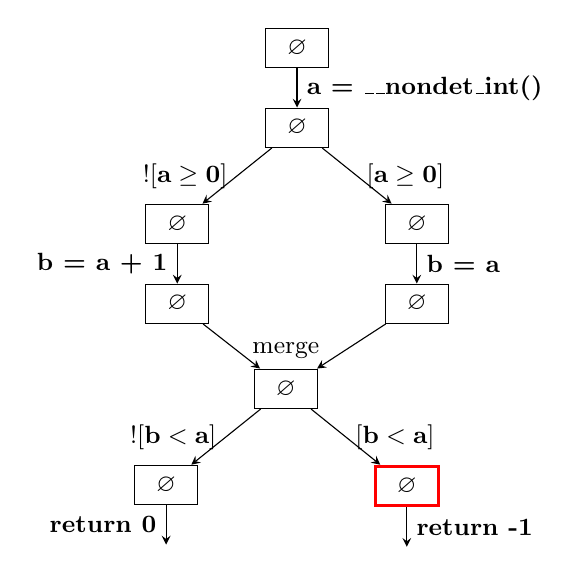
\begin{tikzpicture}[->,>=stealth, mynode/.style={rectangle, draw, minimum height=0.5cm, minimum width=0.8cm}, every node/.style={font=\small}]

  \node[mynode] (0) {$\varnothing$};
  \node[mynode] (1) [below = 0.5cm of 0]{$\varnothing$};
  \node[mynode] (2) [below left = 1cm of 1]{$\varnothing$};
  \node[mynode] (4) [below right = 1cm of 1]{$\varnothing$};
  \node[mynode] (3) [below = 0.5cm of 2]{$\varnothing$};
  \node[mynode] (5) [below = 0.5cm of 4]{$\varnothing$};
  \node[mynode] (6) [below right = 0.8cm of 3, label=north:merge]{$\varnothing$};
  \node[mynode] (7) [below left = 1cm of 6]{$\varnothing$};
  \node[mynode] (8) [below right = 1cm of 6, draw=red, very thick]{$\varnothing$};
  \coordinate[below = 0.5cm of 7] (e7);
  \coordinate[below = 0.5cm of 8] (e8);

  \path
    (0) edge node [right] {\textbf{a = \_\_nondet\_int()}} (1)
    (1) edge node [left, pos=0.5] {$\mathbf{![a \geq 0]}$} (2)
    (1) edge node [right, pos=0.5] {$\mathbf{[a \geq 0]}$} (4)
    (2) edge node [left] {\textbf{b = a + 1}} (3)
    (4) edge node [right] {\textbf{b = a}} (5)
    (3) edge (6)
    (5) edge (6)
    (6) edge node [left, pos=0.5] {$\mathbf{![b < a]}$} (7)
    (6) edge node [right, pos=0.5] {$\mathbf{[b < a]}$} (8)
    (7) edge node [left] {\textbf{return 0}} (e7)
    (8) edge node [right] {\textbf{return -1}} (e8)
  ;
\end{tikzpicture}
%\label{fig:ex1ValueGraph}
%\caption{Analysis of the program to the left by the \valueAnalysisCPA.}
\end{subfigure}
\caption{Simple program and its execution by the \valueAnalysisCPA.}
\label{fig:ex1}
\end{figure}

\begin{figure}[t]
\centering
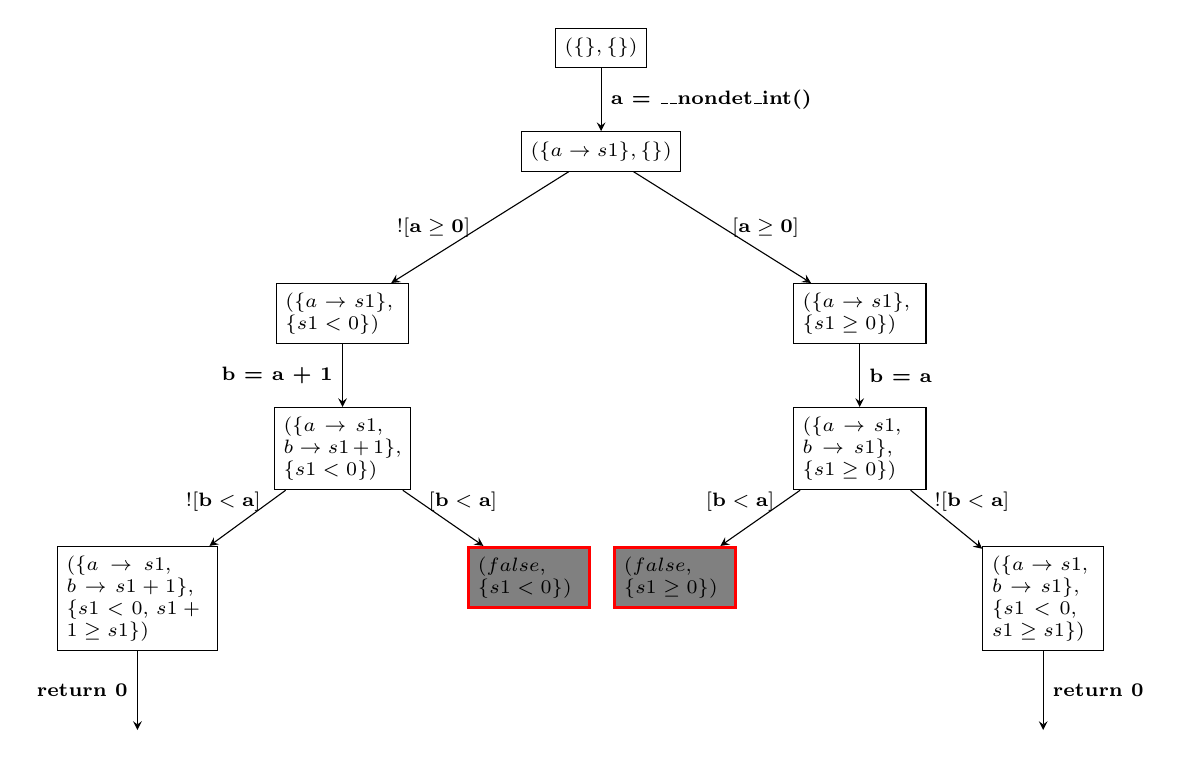
\begin{tikzpicture}[->,>=stealth, mynode/.style={rectangle, draw, minimum height=0.5cm, minimum width=0.8cm}, every node/.style={font=\scriptsize}]

  \node[mynode] (0) {$(\{\}, \{\})$};
  \node[mynode] (1) [below = 0.8cm of 0] {$(\{a \rightarrow s1\}, \{\})$};
  \node[mynode] (2) [below left = 2cm of 1, text width=1.45cm] {$(\{a \rightarrow s1\}$, $\{s1 < 0\})$};
  \node[mynode] (4) [below right = 2cm of 1, text width=1.45cm] {$(\{a \rightarrow s1\}$, $\{s1 \geq 0\})$};
  \node[mynode] (3) [below = 0.8cm of 2, text width=1.5cm] {$(\{a \rightarrow s1$, $b \rightarrow s1+1\}$, $\{s1 < 0\})$};
  \node[mynode] (5) [below = 0.8cm of 4, text width=1.45cm] {$(\{a \rightarrow s1$, $b \rightarrow s1 \}$, $\{s1 \geq 0\})$};
%  \node[mynode] (6) [below = 0.8cm of 3, text width=1.45cm] {$(\{a \rightarrow s1$, $b \rightarrow s1+1\}$, $\{s1 < 0\})$};
 % \node[mynode] (6n) [below = 0.8cm of 5, text width=1.45cm] {$(\{a \rightarrow s1$, $b \rightarrow s1 \}$, $\{s1 \geq 0\})$};
  \node[mynode] (7) [below left = 1cm of 3, text width=1.8cm] {$(\{a \rightarrow s1$, $b \rightarrow s1+1\}$, $\{s1 < 0$, $s1+1 \geq s1\})$};
  \node[mynode] (8) [below right = 1cm of 3, draw=red, fill=gray, very thick, text width=1.3cm]{$(false$, $\{s1 < 0\})$};
  \node[mynode] (8n) [below left = 1cm of 5, draw=red, fill=gray, very thick, text width=1.3cm]{$(false$, $\{s1 \geq 0\})$};
  \node[mynode] (7n) [below right = 1cm of 5, text width=1.3cm] {$(\{a \rightarrow s1$, $b \rightarrow s1\}$, $\{s1 < 0$, $s1 \geq s1\})$};
  \coordinate[below = 1cm of 7] (e7);
  \coordinate[below = 1cm of 7n] (e7n);

  \path
    (0) edge node [right] {\textbf{a = \_\_nondet\_int()}} (1)
    (1) edge node [left, pos=0.5] {$\mathbf{![a \geq 0]}$} (2)
    (1) edge node [right, pos=0.5] {$\mathbf{[a \geq 0]}$} (4)
    (2) edge node [left] {\textbf{b = a + 1}} (3)
    (4) edge node [right] {\textbf{b = a}} (5)
%    (3) edge (6)
%    (5) edge (6n)
    (3) edge node [left, pos=0.2] {$\mathbf{![b < a]}$} (7)
    (3) edge node [right, pos=0.2] {$\mathbf{[b < a]}$} (8)
    (5) edge node [left, pos=0.2] {$\mathbf{[b < a]}$} (8n)
    (5) edge node [right, pos=0.2] {$\mathbf{![b < a]}$} (7n)
    (7) edge node [left] {\textbf{return 0}} (e7)
    (7n) edge node [right] {\textbf{return 0}} (e7n)
  ;
\end{tikzpicture}
\caption{Analysis of the program in Listing \ref{lst:exProg} by the \symbolicExecutionCPA.}
\label{fig:ex1SymExGraph}
\end{figure}

%\subsubsection{Basic Value Analysis can't deal with non-deterministic values (+ Example)}
Figure \ref{fig:ex1} displays an example program that uses non-deterministic values and its analysis using the classic \valueAnalysisCPA.
Since the CPA does not store any information about non-deterministic assignments, no information about the relation between \textbf{a}\ and \textbf{b}\ exists and the property violation is reachable according to the analysis. This produces a \emph{false alarm}.
In constrast to this, the \symbolicExecutionCPA\ is able to handle the non-deterministic assignment to \textbf{a}\ a and its later usage. It returns that the program is safe, correctly.
Figure \ref{fig:ex1SymExGraph} shows this analysis. 

\SymbolicExecutionCPA's ability to track non-deterministic values is able to reduce the number of false alarms to a great extent, as we already showed in \cite{Lemberger2015}.
%\subsubsection{But symbolic value analysis pretty slow, as previous evaluation has shown (illustrate path explosion, sat checks)}
Runtime wise, it performs poorly, though, when compared to the \valueAnalysisCPA.
Since it considers all variable assignments, both deterministic and non-deterministic, and all occurring assumptions, its state space is exponential to the amount of occuring assumptions.
If a infinite loop occurs, the state space is infinite, too.
This problem is called \emph{path explosion}.\cite{Anand2008}
Obviously, an exponential amount of states does not scale to large programs.
In addition, the cost for SAT checks, which are performed at every assumption, are exponential to the amount of non-deterministic values occuring in all encountered assumptions on the currently considered program path.
Evaluation in \cite{Lemberger2015} showed that the \symbolicExecutionCPA\ spends up to 95\% of its runtime for SAT checks.

%\subsubsection{Goal: Try to speed up}
In this work we design, implement and evaluate different approaches to increasing the performance of the \symbolicExecutionCPA.
Our main contribution is, along with variations to the existing merge and less-or-equal operators of the CPA,
the application of CEGAR \cite{Clarke2003} to the composition of the two strongly intertwined CPAs \valueAnalysisCPA\ and \constraintsCPA\ with precision refinement for both CPAs
with two different precision types.

This work is divided into four parts: Theoretical background and contributions, their implementation, their evaluation, and future work and a conclusion.
First we will describe the concepts that are the basis for our work, such as Configurable Software Verification, used CPAs and CEGAR.
Next, we will illustrate the theory behind our own contribution,
before explaining details about the existing and newly added implementation and deviations from theory.
We will evaluate all presented concepts and compare them to the performance of the \valueAnalysisCPA, \predicateCPA, and \symbolicExecutionCPA\ of our old work.
Last, we will give a short outlook to possible future work in this field and close with a conclusion.
%%%%%%%%%%%%%%%%%%%%%%%%%%%%%%%%
\section{Introduction}
%\subsubsection{Why Software Verification is important/needed}
Software systems are prone to error due to multiple factors: The developers skills, humans' limited understanding of software principles, communication problems in development, missing or sparse documentation and unforeseen interdependencies between software components are just some of them.

Because of this testing has been an integral part of software development for quite some time, often claiming about 50\% of development effort and more than 50\% of the budget.
\emph{Software testing} describes the execution of a program with the intention of finding errors.
The tester, either a person or another program, uses different inputs and checks that the proper output is produced.
The nature of this approach determines that only a finite amount of inputs is possible in finite time.
As a result, it is impossible to ensure the errorless execution of a program with arbitrary input.
Additionally, human testing is a technique only shortly touched in most software engineering educations, resembling art more than science.\cite{Myers2011}

Along with these points, the rise of ubiquitious computing and reactive systems complicates the process of reliable verification by testing even more.
Always running systems that gather, evaluate and adapt their behaviour to information of their environment pose an immense amount of possible inputs and interactions due to these.
This makes it almost impossible to predict the behaviour of such systems through testing.

An alternative to testing is formal verification, which tries to produce formal statements that are true for all possible behaviours of a system, using mathematical methods.
These statements are then used for proving that a specific specification is met.
One area of formal verification is \emph{automated software verification}. It tries to reach the above goal by only using software that works without the help or feedback of humans.
\CpaChecker\ \cite{Beyer2011} is such a program that yielded excellent performance in the last iterations of  the \href{http://sv-comp.sosy-lab.org}{Competition on Software Verification} (SV-COMP) \cite{SV-COMP2013} \cite{SV-COMP2014} \cite{SV-COMP2015}.
\CpaChecker\ is a framework for \emph{Configurable Software Verification} \cite{Beyer2007} utilizing different \emph{configurable program analyses} (CPAs) to locate possible property violations of a specification in a program.
Three such CPAs are the \valueAnalysisCPA, which uses concrete variable assignments, the \predicateCPA, which creates predicates for describing properties of program paths,
and the \symbolicExecutionCPA, which uses an extension of the \valueAnalysisCPA\ tracking non-deterministic values as symbolic ones in combination with the \constraintsCPA, which tracks constraints to symbolic values on program paths.
While the \valueAnalysisCPA\ has high efficiency due to her simplicity, it can't handle complex program characteristics like pointers or non-deterministic values.
The \predicateCPA, in constrast, is very expressive, but has low efficiency since SAT checks are necessary for computing the feasibility of a program path.
The \symbolicExecutionCPA\ poses something in between those two, not being able to handle some complex program characteristics as it is partly based on the \valueAnalysisCPA, but being able to handle non-deterministic values.
On the other hand, it uses SAT checks, too, though less often and over smaller formulas.

\begin{figure}[t]
\lstset{numbers=left}
\begin{subfigure}[b]{.45\textwidth}
\lstinputlisting[language=C]{exampleProgram.c}
%\caption{A simple non-deterministic program.}
%\label{lst:exProg}
\end{subfigure}%
\hfill
\begin{subfigure}[b]{.45\textwidth}
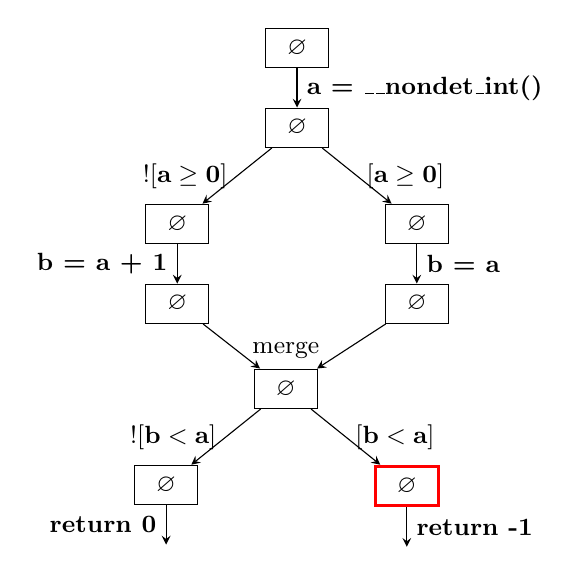
\begin{tikzpicture}[->,>=stealth, mynode/.style={rectangle, draw, minimum height=0.5cm, minimum width=0.8cm}, every node/.style={font=\small}]

  \node[mynode] (0) {$\varnothing$};
  \node[mynode] (1) [below = 0.5cm of 0]{$\varnothing$};
  \node[mynode] (2) [below left = 1cm of 1]{$\varnothing$};
  \node[mynode] (4) [below right = 1cm of 1]{$\varnothing$};
  \node[mynode] (3) [below = 0.5cm of 2]{$\varnothing$};
  \node[mynode] (5) [below = 0.5cm of 4]{$\varnothing$};
  \node[mynode] (6) [below right = 0.8cm of 3, label=north:merge]{$\varnothing$};
  \node[mynode] (7) [below left = 1cm of 6]{$\varnothing$};
  \node[mynode] (8) [below right = 1cm of 6, draw=red, very thick]{$\varnothing$};
  \coordinate[below = 0.5cm of 7] (e7);
  \coordinate[below = 0.5cm of 8] (e8);

  \path
    (0) edge node [right] {\textbf{a = \_\_nondet\_int()}} (1)
    (1) edge node [left, pos=0.5] {$\mathbf{![a \geq 0]}$} (2)
    (1) edge node [right, pos=0.5] {$\mathbf{[a \geq 0]}$} (4)
    (2) edge node [left] {\textbf{b = a + 1}} (3)
    (4) edge node [right] {\textbf{b = a}} (5)
    (3) edge (6)
    (5) edge (6)
    (6) edge node [left, pos=0.5] {$\mathbf{![b < a]}$} (7)
    (6) edge node [right, pos=0.5] {$\mathbf{[b < a]}$} (8)
    (7) edge node [left] {\textbf{return 0}} (e7)
    (8) edge node [right] {\textbf{return -1}} (e8)
  ;
\end{tikzpicture}
%\label{fig:ex1ValueGraph}
%\caption{Analysis of the program to the left by the \valueAnalysisCPA.}
\end{subfigure}
\caption{Simple program and its execution by the \valueAnalysisCPA.}
\label{fig:ex1}
\end{figure}

\begin{figure}[t]
\centering
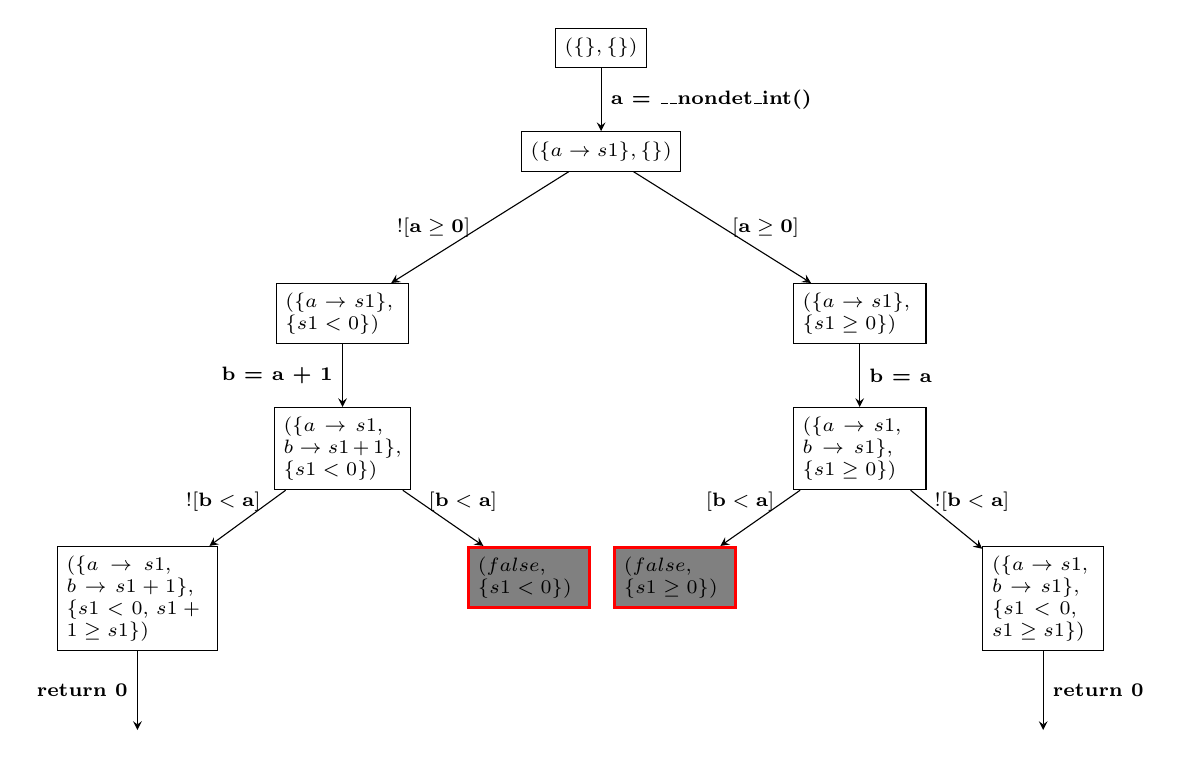
\begin{tikzpicture}[->,>=stealth, mynode/.style={rectangle, draw, minimum height=0.5cm, minimum width=0.8cm}, every node/.style={font=\scriptsize}]

  \node[mynode] (0) {$(\{\}, \{\})$};
  \node[mynode] (1) [below = 0.8cm of 0] {$(\{a \rightarrow s1\}, \{\})$};
  \node[mynode] (2) [below left = 2cm of 1, text width=1.45cm] {$(\{a \rightarrow s1\}$, $\{s1 < 0\})$};
  \node[mynode] (4) [below right = 2cm of 1, text width=1.45cm] {$(\{a \rightarrow s1\}$, $\{s1 \geq 0\})$};
  \node[mynode] (3) [below = 0.8cm of 2, text width=1.5cm] {$(\{a \rightarrow s1$, $b \rightarrow s1+1\}$, $\{s1 < 0\})$};
  \node[mynode] (5) [below = 0.8cm of 4, text width=1.45cm] {$(\{a \rightarrow s1$, $b \rightarrow s1 \}$, $\{s1 \geq 0\})$};
%  \node[mynode] (6) [below = 0.8cm of 3, text width=1.45cm] {$(\{a \rightarrow s1$, $b \rightarrow s1+1\}$, $\{s1 < 0\})$};
 % \node[mynode] (6n) [below = 0.8cm of 5, text width=1.45cm] {$(\{a \rightarrow s1$, $b \rightarrow s1 \}$, $\{s1 \geq 0\})$};
  \node[mynode] (7) [below left = 1cm of 3, text width=1.8cm] {$(\{a \rightarrow s1$, $b \rightarrow s1+1\}$, $\{s1 < 0$, $s1+1 \geq s1\})$};
  \node[mynode] (8) [below right = 1cm of 3, draw=red, fill=gray, very thick, text width=1.3cm]{$(false$, $\{s1 < 0\})$};
  \node[mynode] (8n) [below left = 1cm of 5, draw=red, fill=gray, very thick, text width=1.3cm]{$(false$, $\{s1 \geq 0\})$};
  \node[mynode] (7n) [below right = 1cm of 5, text width=1.3cm] {$(\{a \rightarrow s1$, $b \rightarrow s1\}$, $\{s1 < 0$, $s1 \geq s1\})$};
  \coordinate[below = 1cm of 7] (e7);
  \coordinate[below = 1cm of 7n] (e7n);

  \path
    (0) edge node [right] {\textbf{a = \_\_nondet\_int()}} (1)
    (1) edge node [left, pos=0.5] {$\mathbf{![a \geq 0]}$} (2)
    (1) edge node [right, pos=0.5] {$\mathbf{[a \geq 0]}$} (4)
    (2) edge node [left] {\textbf{b = a + 1}} (3)
    (4) edge node [right] {\textbf{b = a}} (5)
%    (3) edge (6)
%    (5) edge (6n)
    (3) edge node [left, pos=0.2] {$\mathbf{![b < a]}$} (7)
    (3) edge node [right, pos=0.2] {$\mathbf{[b < a]}$} (8)
    (5) edge node [left, pos=0.2] {$\mathbf{[b < a]}$} (8n)
    (5) edge node [right, pos=0.2] {$\mathbf{![b < a]}$} (7n)
    (7) edge node [left] {\textbf{return 0}} (e7)
    (7n) edge node [right] {\textbf{return 0}} (e7n)
  ;
\end{tikzpicture}
\caption{Analysis of the program in Listing \ref{lst:exProg} by the \symbolicExecutionCPA.}
\label{fig:ex1SymExGraph}
\end{figure}

%\subsubsection{Basic Value Analysis can't deal with non-deterministic values (+ Example)}
Figure \ref{fig:ex1} displays an example program that uses non-deterministic values and its analysis using the classic \valueAnalysisCPA.
Since the CPA does not store any information about non-deterministic assignments, no information about the relation between \textbf{a}\ and \textbf{b}\ exists and the property violation is reachable according to the analysis. This produces a \emph{false alarm}.
In constrast to this, the \symbolicExecutionCPA\ is able to handle the non-deterministic assignment to \textbf{a}\ a and its later usage. It returns that the program is safe, correctly.
Figure \ref{fig:ex1SymExGraph} shows this analysis. 

\SymbolicExecutionCPA's ability to track non-deterministic values is able to reduce the number of false alarms to a great extent, as we already showed in \cite{Lemberger2015}.
%\subsubsection{But symbolic value analysis pretty slow, as previous evaluation has shown (illustrate path explosion, sat checks)}
Runtime wise, it performs poorly, though, when compared to the \valueAnalysisCPA.
Since it considers all variable assignments, both deterministic and non-deterministic, and all occurring assumptions, its state space is exponential to the amount of occuring assumptions.
If a infinite loop occurs, the state space is infinite, too.
This problem is called \emph{path explosion}.\cite{Anand2008}
Obviously, an exponential amount of states does not scale to large programs.
In addition, the cost for SAT checks, which are performed at every assumption, are exponential to the amount of non-deterministic values occuring in all encountered assumptions on the currently considered program path.
Evaluation in \cite{Lemberger2015} showed that the \symbolicExecutionCPA\ spends up to 95\% of its runtime for SAT checks.

%\subsubsection{Goal: Try to speed up}
In this work we design, implement and evaluate different approaches to increasing the performance of the \symbolicExecutionCPA.
Our main contribution is, along with variations to the existing merge and less-or-equal operators of the CPA,
the application of CEGAR \cite{Clarke2003} to the composition of the two strongly intertwined CPAs \valueAnalysisCPA\ and \constraintsCPA\ with precision refinement for both CPAs
with two different precision types.

This work is divided into four parts: Theoretical background and contributions, their implementation, their evaluation, and future work and a conclusion.
First we will describe the concepts that are the basis for our work, such as Configurable Software Verification, used CPAs and CEGAR.
Next, we will illustrate the theory behind our own contribution,
before explaining details about the existing and newly added implementation and deviations from theory.
We will evaluate all presented concepts and compare them to the performance of the \valueAnalysisCPA, \predicateCPA, and \symbolicExecutionCPA\ of our old work.
Last, we will give a short outlook to possible future work in this field and close with a conclusion.

\bibliographystyle{acm}
\bibliography{softwareVerification}

\end{document}
